% ustawienia dokumentu dla Windows
\UseRawInputEncoding 

\documentclass{article}
\usepackage{hyperref}
\usepackage{listings}
\usepackage{graphicx}	% do tabelki żeby centrować
\usepackage{longtable}	% podział tabeli między strony, nie jest uzyte
\usepackage{placeins}	% wymuszenie tekstu za tabelką
\title{Python Notes}
\author{anana}
\date{2022-09-06}

% Poszerzenie strony
\usepackage{geometry}
\newgeometry{vmargin={25mm}, hmargin={25mm,25mm}}


% definicje kolorów
\usepackage{color}
\definecolor{pythonlexis}{RGB}{200,100,0}
\definecolor{pythoncomment}{RGB}{0,80,0}
\definecolor{pythonerror}{RGB}{150,0,0}

% definicja 

% styl dla kodu python
% wiecej opcji https://nasa.github.io/nasa-latex-docs/html/examples/listing.html
\lstdefinestyle{pystyle}
{   numberblanklines=false,
    language=Python,
    tabsize=4,
    breaklines=true,
    basicstyle=\small,
    keywordstyle=\color{pythonlexis},
    commentstyle=\color{pythoncomment}\upshape,
}

% styl dla BASH
\lstdefinestyle{bash}
{   numberblanklines=false,
    language=bash,
    tabsize=4,
    breaklines=true,
    basicstyle=\small,
    commentstyle=\color{pythoncomment}\upshape,
}

\begin{document}
	\pagenumbering{gobble}
	\maketitle

	\newpage
	\pagenumbering{arabic}
	\tableofcontents
	
	\newpage
	\section{Basic Of Python}
	In this section you will find basic information about programming languages and introduction to Python language.
	\subsection{General Language Information}
	\subsubsection{What Makes Language}
	Each language (human and computer) consist of the following elements:
	\begin{itemize}
	\item ALPHABET - set of symbols used to build words. Programming languages usualy base on Latin alphabet.
	\item LEXIS - or dictionary - simple list of words which has some meaning.
	\item SYNTAX - set of rules determining the words combination has sense. Syntax errors are detected by compiler / interpreter.
	\item SEMANTICS - set of rules detrmining sytax has sense. Semantics errors are detected by programmers during code review. E.g.: we expecting a sum of two numbers but the result is a sum of two strings.
	\begin{lstlisting}[language=Python]
	a = input()
	print(a + a)
	\end{lstlisting}
	\end{itemize}
	\subsubsection{HLPL and LLPL}
	HLPL - High Level Programming Languages - are easly understandable by humans, while LLPL - Low Level Programming Languages are those more friendly for machines. 
	\paragraph{}
	Ususally HLPL are easier to understand, code and debug. Can be easly ported to different computer architectures and can be run on any platform. They need interpreter, complirer or translator - a tool which perform translation from HLPL to form which is understandable by machine. Examples of HLPL: C, C++, Java, Python, JavaScript.
	\paragraph{}
	On the other hand LLPL are usualy hard to understand for human, therefore hard to develop and debug. Usually are closly dependednt on HW. They still need a tool - assembler to be translated to machine code (assembler language). This kind of development is kindly usefull in solution where high efficient or limited resources matter. Examples of LLPL: assembly language, machine language.
	\begin{itemize}
	\item SOURCE CODE - it is file containing code written by developer in HLPL.
	\item COMPILER - a tool wchich read source code and turns it into assembly or bytecode or machine code.
	\item ASSEMBLY LANGUAGE - low level programming language, which code is understandable for machine or for applications.
	\item BYTECODE - low level code understandable for application, e.g. virtual machine of specific language.
	\item MACHINE CODE - binary representation of code which can be run on HW directly. Consist of zeros and ones. Can be understand only by CPU. 
	\end{itemize}
	\subsubsection{Compiler and Interpreter}
	\paragraph{}
	Source code written in HLPL is a file containing instruction which uses words or phrases easy understandable by human. To execute this code on machine it must be first translated to form which machine can understand. The proces of tranlating source code to machine code is performing by programs called interpreters or compilers.
	\paragraph{}
	During compilation the source code is translated only once - compiler scan whole source code and translate it into machine code. But after each, even smaller change in code the compilation must be repeated. Produced executable is ready to distribute as is, can be run on desired machine, no any other programs are required. Compilation process might be very long - it depend of project/program complexity. Compliler report error after scanning process of whole source code, this sometimes makes debugging harder. Worth to note that compliers does not translate source code to binary code directly but generate also intermediary objects, and linking process is needed.
	\paragraph{}
	During interpretation the source code (script) need to be run by interpreter, each line of source code is translated at time. Interpreter doing it fast (does not generate intermediary objects). Translation is stopped when first error appears in source code line. Interpreter must be installed on the machine. Without the interpreter it is not possible to run the source code. Interpreter is fast, but overall time to execute the process is much slower compared to binary execution of compiled program.
	
	
	\newpage
	\subsection{Versions of Python}
	Different Python implementations exist.
	\begin{itemize}
	\item CPython - canonical or reference Python.Written in C language.
	\item Cython - combination of C language and Python.
	\item Jthon - Java implementation of Python.
	\item PyPy and Ppython - Python for Python, restricted. It is used mainly as tool for developing of Python, as some things are easier perform in Python than in pure C language.
	\end{itemize}
	\paragraph{}
	Python3 is not compatible with older version Python2.
	\paragraph{}
	Python is not suitable for low level programming - bare metal devices, hardware with limited computing resources. It is also not suitable for mobile device application.
	\paragraph{}
	Python can be successfully used in Web service development, PC applications, test sctipting, simulations, data analysis, AI.
	\paragraph{}
	Python is distributed by default with the standard library which is very extensive and provides users with a wide range of facilities.
	
	\newpage
	\subsection{Built-in Functions}
	Basic built-in function available with Python installation are:
	\begin{itemize}
	\item print()
	\item dir()
	\item input()
	\item id()
	\item type()
	\item pow()
	\item upper()
	\item lower()
	\item range()
	\item sorted()
	\end{itemize}
	\subsubsection{Built-in function: print()}
	This is one most popular function which allows to communicate our script with us - it prints information to standard output by default (to console output). It accepts five arguments, but usually is used only with one argument - objects:
	\begin{lstlisting}[style=pystyle]
print(*objects, sep=' ', end='\n', file=sys.stdout, flush=False)
	\end{lstlisting}
	This function accept all python objects and return None.
	Listening below shows few unusuall print function calls with their outputs:
	\begin{lstlisting}[style=pystyle]
# no arguments means that only default end="\n" is printing
print()

# print can accept single quotation mark as well as double quotation mark
print("")
print('')

# Provide object separated by comma. Default separator cause that space is included after each printed object
print("Ala", 1, 2, "", 3)	#'Ala 1 2  3'
# Modify default separator to different char
print(1, 2, 3, sep="+")		#'1+2+3'
# Modify default last new line character to different 
print('Kot means cat', end='\nKICIA*\n')
#Kot means cat
#KICIA*
	\end{lstlisting}
	The \textbf{flush} parameter determine usage of system buffers for buffering data which we want to sent to stream. Default value is False and it means stream is buffered - data is collecting in buffer and later printing / sending to stream. this increase performance of print function. Setting flush to True we disabling the buffering, and every single character is printing immedietly to our defined output, without buffer. In this case print function is calling many times which is affecting performance. In print function flush configuration take effect if end parameter is set to something different than "n".
	\begin{lstlisting}[style=pystyle]
import time
for i in range(4):
    print(i, end=" - ", flush=True)
    time.sleep(1)
# Will print each i separatelly every second
for i in range(4):
    print(i, end=" - ", flush=False)
    time.sleep(1)
# Will print all i values at once at the end after 4 seconds
	\end{lstlisting}
	The last parameter \textbf{file} determine output (stream) where print redirect data. Default it is set to sys.stdout - standart output for particular system. It can be changed for another stream, e.g. to file. The file must be created and opened before redirection, this is why we use open - another one built in function.:
	\begin{lstlisting}[style=pystyle]
import datetime
with open("my_text_file.txt", "a") as this_file:
    print(datetime.datetime.now(), end=": ", file=this_file)
    for i in range(4):
        print(i, end=" - ", file=this_file)
    print(file=this_file)
# Every print call has defined file where the data will be redirected and stored. 
	\end{lstlisting}
	
	\subsubsection{Built-in function: sorted()}
	It takes any iterable, sort it and return elements as list. It takes 3 parameters, where only first is mandatory: 
	\begin{lstlisting}[style=pystyle]
sorted(iterable, /, *, key=None, reverse=False)

# Sort integers
sorted([4,32,5,43])			#[4, 5, 32, 43] 
# Sort characters
sorted(['b', 'B', 'A', 'a'])#['A', 'B', 'a', 'b'] 
# Sort elements of string
sorted("ala ma")			#[' ', 'a', 'a', 'a', 'l', 'm']
	\end{lstlisting}
	Second parameter of this function is a \textbf{key} which define the way how sorting shold be prform. The key can be a function. Last parameter is \textbf{reverse} boolean determining the sorting order. 
	\begin{lstlisting}[style=pystyle]
# Sort integers and characters together
sort_func=lambda data: (isinstance(data, int), data)
sorted(['b', 4, 'a', 1, -1, 2], key=sort_func)	#['a', 'b', -1, 1, 2, 4]
	\end{lstlisting}
	
	
	\subsubsection{Built-in function: map()}
	It takes 2 or more arguments - a function and any iterable. It applies the function for each element from collection and returns a map object which is actually an interator.  
\begin{lstlisting}[style=pystyle]
map(fun, *iter)

map(lambda x: x + x, [1, 2, 3])	#2, 4, 6
map(lambda x, y: x - y, (1, 2, 3), (6, 5, 6))	#-5, -3, -3
map(lambda x:round(math.sin(x), 2), [1, 2, 3])	#0.84, 0.91, 0.14
\end{lstlisting}
	

	\subsubsection{Built-in function: filter()}
	It takes 2 or more arguments - a function and any iterable. The function has a role of filter, determining which elements from provided sequence will be returned.  
\begin{lstlisting}[style=pystyle]
filter(fun, iter)

filter(lambda x: x<3, [1,2,3])	#1, 2
\end{lstlisting}


	\subsubsection{Built-in function: dir()}
Without arguments, return the list of names in the current local scope. With an argument, attempt to return a list of valid attributes for that object.
	\begin{lstlisting}[style=pystyle]
# Print all items inside math module
import math
print(dir(math))

# Print all items in local scope
print(dir())
	\end{lstlisting}
The dir function calls \_\_dir\_\_() method.
	\begin{lstlisting}[style=pystyle]
class Ala:
    gender = "female"
    def __init__(self, name):
        self.name = name
        self.age = 1
    def age(self):
        return self.age

a = Ala(1)
dir(a)
dir(Ala(2))
# content of dir(Ala(2)) and dir(a) is the same. 
	\end{lstlisting}



	\newpage
	\subsection{Built-in Types}
	Built-in type are types which are always available in python installation and we do not have to import them. Basic build-in types are:
	\begin{itemize}
	\item numerics
	\item sequences
	\item mappings
	\item classes
	\item instances
	\item exceptions
	\item modules
	\item functions
	\item methods
	\item code objects
	\item type objects
	\item Null object
	\item Ellipsis object
	\item NotImplemented object
	\item booleans
	\end{itemize}
	This is only generalised list of built-in types. To see each available built-int type provided by python run code:
	\begin{lstlisting}[style=pystyle]
import builtins as bi
bitypeslist = [bit for bit in bi.__dict__.values() if isinstance(bit, type)]
for item in bitypeslist:
    print(item)
	\end{lstlisting}
	
	Built-in are not python keywords, it means it is possible to use buit-in names for variable, which is strongly not recommended, and may lead to errors in code:
	\begin{lstlisting}[style=pystyle]
bool="ala"
bool(1)
Traceback (most recent call last):
  File "<stdin>", line 1, in <module>
TypeError: 'str' object is not callable
del(bool)
bool(1)
True
	\end{lstlisting}
Some python objects are \textbf{muttable} - they rearrange their members in place. Mutable objects are changeable or has the ability to change (change value, status, state). Other object types are \textbf{immutable} - they cannot be modified, and making change to them a new object is creating. Builtin types which are mutable are:
\begin{itemize}
\item lists
\item sets
\item dictionaries
\end{itemize}
Builtin types which are immutable are:
\begin{itemize}
\item numbers
\item strings
\item tuples
\item frozen sets
\end{itemize}
Object mutability is a characteristics which make Python a \textbf{dynamically typed language}. 
	In sections below selected types will be covered.
	

	\subsubsection{Built-in types: numerics}
	In Python are three different numeric types:
	\begin{itemize}
	\item integers
	\item floating point numbers
	\item complex numbers
	\end{itemize}
	\paragraph{}
	Integers have unlimited precission (it is limited only by machine on which Python is running). Integers can be used and represented in different manner:
	\begin{lstlisting}[style=pystyle]
print(123)		#123
print(1_2_3)	#123
print(+111)		#111
print(+0)		#0
print(-0)		#0
print(--123)	#123
print(-123)		#-123 
print(---123)	#-123 
print(-+-+-123)	#-123
	\end{lstlisting}

	\paragraph{}
	Floating point numbers are implemented using C language double data type. To get information about limits on current machine call $sys.float\_info$. For my machine it produces following data:
	\begin{lstlisting}[style=pystyle]
import sys
sys.float_info
sys.float_info(max=1.7976931348623157e+308, max_exp=1024, max_10_exp=308, min=2.2250738585072014e-308, min_exp=-1021, min_10_exp=-307, dig=15, mant_dig=53, epsilon=2.220446049250313e-16, radix=2, rounds=1)
	\end{lstlisting}
	Floats can be used and represented in different manner:
	\begin{lstlisting}[style=pystyle]
print(.123)		#0.123
print(1_2_3.4)	#123.4
print(+111.00)	#111.0
print(3.)		#3.0
print(-03.0)	#-3.0
print(-0.)		#-0.0
print(-.000)	#-0.0 
print(+0.0)		#0.0
# Zero and minus zero are equal
print(0==-.0000)	#True
# Representing floating point in scientific notation (E, e)
print(1e3)		#1000.0
print(1e-3)		#0.001
print(-1.e-2)	#-0.01
print(1.E2)		#100.0
print(0.E3)		#0.0
	\end{lstlisting}
	As you can see \textbf{negative zero -0} and \textbf{possitive zero +0} are supported by Python. Their values are equal, but for some application the sign might be used.
	\paragraph{}
	Complex numbers which have real and imaginary part, they base on floating point number. Assuming $z$ is complex number, real part can be accessed $z.real$, and imaginary $z.imag$.
	

	\subsubsection{Built-in types: str (text sequence)} 
	Python str (string) is a textual data type. Strings are immutable (cannot be updated) sequences of Unicode code points. Strings can be put in single quotes, double quotes or tripple quotes (these can span multiple lines). In multi line strings new line character is invisible but present. This means 'empty' multi line string will have size equal to number of lines.
	\paragraph{}
	While single char data is not existing in Python each single character is actually single string. Thus, assuming $s$ is a not empty string: $s[0] == s[0:1]$.
	\paragraph{}
	Empty string length is equal to zero. Thus empty string is interpreted as $False$.
	\paragraph{}
	Strings are sequences, and can be treated like lists in many particular cases. Below are presented typical operations on strings:
\begin{itemize}
\item \textbf{concatenation} - join by + operator
\item \textbf{replication} - multiplication by * operator. Replication by 0 or negative values result wit empty string. Replication is allowed only by using integers. Attempt to use e.g. float number ends with \textcolor{pythonerror}{TypeError: can't multiply sequence by non-int of type 'float'} error.
	\begin{lstlisting}[style=pystyle]
# Strings can be added (concatenaded)
"" + ' ' + "33" + ' rota'	#' 33 rota'
# String can be multipled by a number.
# Positive number duplicate string (replicated)
"Ala "*2	#'Ala Ala '
# Zero or nrgative number creates empty string
"Ala" * 0	#''
	\end{lstlisting}
\item  \textbf{comparison} - compares code point values, character by character. If both strings are identical, but one is longer than another it also matter.
\begin{lstlisting}[style=pystyle]
"ala" == "ala"	#True
"ala" == "alA"	#False
"ala " == "ala"	#False
"ala" != "ala"	#False
"ala" > "ala"	#False
"ala" < "ala"	#False
"ala" >= "ala"	#True
"ala" <= "ala"	#True
"ala " > "ala"	#True
"ala" > "Ala"	#True
"Ala" > "ala"	#False
\end{lstlisting}
Comparing strings with number is possible but WRONG. Only \textbf{==} and \textbf{!=} operators are allowed, and comparison with == always produce False, while comparison with != always produce True. Attempt to use $<, <=, >, >=$ operators ends with \textcolor{pythonerror}{TypeError}
\item \textbf{ord(str)} (ordinal - porzadkowy) - returns ASCII/Unicode number (code point) representing character. The function needs a one-character string as its argument - breaching this requirement causes a \textcolor{pythonerror}{TypeError} exception, and returns a number representing the argument's length.	
\item \textbf{chr(int)} - this function takes a code point and returns its character. \textcolor{pythonerror}{TypeError} is raised when trying pass anything different than integer. \textcolor{pythonerror}{ValueError} is raising in case of negative integers.
\item len("some string")
\item indexing
\item slicing
\begin{lstlisting}[style=pystyle]
        #654321 minus
        #012345
alpha = "abdefg"
print(alpha[1:3])   #'bd'
print(alpha[3:])    #'efg'
print(alpha[:3])    #'abd'
print(alpha[3:-2])  #'e'
print(alpha[-3:4])  #'e'
print(alpha[::2])   #'adf'
print(alpha[1::2])  #'beg'
\end{lstlisting}
\item Iterating through the strings
\begin{lstlisting}[style=pystyle]
for s in "kaszanka":
    print(s, end="-")	#k-a-s-z-a-n-k-a-
\end{lstlisting}
\item \textbf{in} or \textbf{not in} - checks if the substring exists or not exists in a string. Returns True or False.
\item \textbf{min(str)} - str cannot be empty. Returns character with smallest value from string based on code point value from ASCII/Unicode table.
\item \textbf{max(str} - str cannot be empty. Returns character with biggest value from string based on code point value from ASCII/Unicode table.
\item \textbf{sorting by sorted() or sort()} - to sort string content sorted() function can be used. To sort list of strings sorted() function or sort() method can be used. The sorted() function takes one argument and returns new sorted list. The sort() methods operate on sorted item (sorted list is upodating in place).
\begin{lstlisting}[style=pystyle]
# sorted()
my_string="bca"
print(sorted(my_string))		#['a', 'b', 'c']
print(my_string)				#bca

# sort()
my_string_list = ["la", "do", "aa", "Ab"]
my_string_list.sort()
print(my_string_list)			#['Ab', 'aa', 'do', 'la'] A > a
\end{lstlisting}
\item \textbf{mapping str numbers} - it is easy to map int or float to string. But converting str to number is complicated, and depend on string content.
\begin{lstlisting}[style=pystyle]
int("-12")				#-12
int("12.1")				#ValueError
float("12.1")			#12.1
float("12e2")			#1200.0
float("12.5454")		#12.5454
float("12.5454\t")		#12.5454
\end{lstlisting}
\item \textbf{list(str)} - convert string to list. Every single character produces separate list element.
\end{itemize}

Strings are immutable, thus some operations are forbiden - like del, append(), insert(). 
\paragraph{}

Sting class privides multiple unique methods. Knowing them is very usefull and save time during development:
\begin{itemize}
\item \textbf{strip(self, chars)} - returns a string with removed chars on both sides of string. By default removes white spaces, but it can be customized.
\begin{lstlisting}[style=pystyle]
" string to modify \t  ".strip()		#'string to modify'
" string to modify \t  ".strip("yfs\t ")#'tring to modi'
\end{lstlisting}

\item \textbf{lstrip(self, chars)} - returns a string with removed chars only from left side of string. By default removes white spaces, but chars can be customized.
\begin{lstlisting}[style=pystyle]
" string to modify \t  ".lstrip()		 #'string to modify \t  '
" string to modify \t  ".lstrip("yfs\t ")#'tring to modify \t  '
\end{lstlisting}

\item \textbf{rstrip(self, chars)} - returns a string with removed chars only from right side of string. By default removes white spaces, but chars can be customized.
\begin{lstlisting}[style=pystyle]
" string to modify \t  ".rstrip()			#' string to modify'
" string to modify \t  ".rstrip("yfs\t ")	#' string to modi'
\end{lstlisting}

\item \textbf{center(self, width, fillchar)} - returns a centered string of lenght width. By default white spaces are used to fill gaps, but chars can be customized.
\begin{lstlisting}[style=pystyle]
" string to modify ".center(25)		#'     string to modify    '
" string to modify ".center(25, '-')#'---- string to modify ---'
\end{lstlisting}

\item \textbf{ljust(self, width, fillchar)} - returns a left justified string of lenght width. By default white spaces are used to fill gaps, but chars can be customized.
\begin{lstlisting}[style=pystyle]
" string to modify ".ljust(25)		#' string to modify        '
" string to modify ".ljust(25, '-')	#' string to modify -------'
\end{lstlisting}

\item \textbf{rjust(self, width, fillchar)} - returns a right justified string of lenght width. By default white spaces are used to fill gaps, but chars can be customized.
\begin{lstlisting}[style=pystyle]
" string to modify ".rjust(25)		#'        string to modify '
" string to modify ".rjust(25, '-')	#'------- string to modify '
\end{lstlisting}

\item \textbf{zfill(self, width)} - returns string padded with zeros.
\begin{lstlisting}[style=pystyle]
"frfr".zfill(12)	#'00000000frfr'
\end{lstlisting}

\item \textbf{lower(self)}, \textbf{upper(self)}, \textbf{capitalize(self)}, \textbf{casefold(self)}, \textbf{title(self)} and \textbf{swapcase(self)} - all these methods return strings with modified character size. The casefold() is more aggressive than lower() method, as it tries to change chras which are the same shape for upper and lower case.
\begin{lstlisting}[style=pystyle]
"STRING to modify".lower()		#'string to modify'
"STRING to modify".upper()		#'STRING TO MODIFY'
"STRING to modify".capitalize()	#'String to modify'
"STRING to modify".casefold()	#'string to modify'
"STRING to modify".swapcase()	#'string TO MODIFY'
"STRING to modify".title()		#'String To Modify'
\end{lstlisting}

\item Group of test methods checking string content. All of them return True or False.
\begin{lstlisting}[style=pystyle]
"String".isupper()			#False
"STRING".isupper()			#True
"String".islower()			#False
"string".islower()			#True
"String".istitle()			#True
" String".istitle()			#False
"String\t".isprintable()	#False
"String".isprintable()		#True
"String".isascii()			#True
"[\x80-\xFF]".isascii()		#False
chr(179).isdecimal()		#False
"123".isdecimal()			#True
chr(179).isdigit()			#True
chr(8558).isdigit()			#False
chr(8558).isnumeric()		#True
"String".isnumeric()		#False
"String".isalpha()			#True
"121212".isalpha()			#False
"String1".isalnum()			#True
"String1\t".isalnum()		#False
" \t\t\t\t".isspace()		#True
"String".isspace()			#False
"String".isidentifier()		#True
"1String".isidentifier()	#False
\end{lstlisting}
Be aware that empty string returns True only in 2 types of tests.
\begin{lstlisting}[style=pystyle]
"".isascii()		#True
"".isprintable()	#True
\end{lstlisting}
The isupper() and islower() are valid only to letters. For other characters reports always False.
And the \textbf{indentifier} in Python is a string containing only following characters: A-Za-z, 0-9, \_

\item \textbf{endswith(self, sufix, indexstart, indexstop)} - returns True if string ends with sufix, otherwise False.
\begin{lstlisting}[style=pystyle]
#0123456789 - indexes
"osa-ma-oko".endswith("ma") 		#False
"osa-ma-oko".endswith("-oko") 		#True
"osa-ma-oko".endswith("-") 			#False
"osa-ma-oko".endswith("-", 5, 7) 	#True
"osa-ma-oko".endswith("-", 5, 6) 	#False
"osa-ma-oko".endswith("-", 5, 8) 	#False
"osa-ma-oko".endswith(("-", "ko")) 	#True
\end{lstlisting}

\item \textbf{startswith(self, sufix, indexstart, indexstop)} - returns True if string starts with sufix, otherwise False.
\begin{lstlisting}[style=pystyle]
#0123456789 - indexes
"osa-ma-oko".startswith("sa") 		#False
"osa-ma-oko".startswith("osa") 		#True
"osa-ma-oko".startswith("osa", 1) 	#False
"osa-ma-oko".startswith("sa", 1) 	#True
\end{lstlisting}

\item \textbf{partition(self, sep)} - returns tupleof 3 elements (part before first sep, sep, part after sep)
\begin{lstlisting}[style=pystyle]
"ffrfrf".partition("4")		#('ffrfrf', '', '')
"ffrfrf".partition("r")		#('ff', 'r', 'frf')
"ffrfrf".partition("f")		#('', 'f', 'frfrf')
\end{lstlisting}

\item \textbf{join(self, iterable)} - returns string from list of strings in iterable joined by predefined join string.
\begin{lstlisting}[style=pystyle]
" ".join(["ala", "ola"])	#'ala ola'
" -- ".join("ala")			#'a -- l -- a'
\end{lstlisting}

\item \textbf{split(self, sep, maxsplit)} - returns list of strings separated by sep. Number of separations are limited to maxsplit (counting from left side)
\begin{lstlisting}[style=pystyle]
"ola1ala1ela1ewa".split()		#['ola1ala1ela1ewa']
"ola1ala1ela1ewa".split("1")	#['ola', 'ala', 'ela', 'ewa']
"ola1ala1ela1ewa".split("1", 2)	#['ola', 'ala', 'ela1ewa']
\end{lstlisting}

\item \textbf{rsplit(self, sep, maxsplit)} - returns list of strings separated by sep. Number of separations are limited to maxsplit (counting from right side)
\begin{lstlisting}[style=pystyle]
"ola1ala1ela1ewa".rsplit()		#['ola1ala1ela1ewa']
"ola1ala1ela1ewa".rsplit("1")	#['ola', 'ala', 'ela', 'ewa']
"ola1ala1ela1ewa".rsplit("1", 2)#['ola1ala', 'ela', 'ewa']
\end{lstlisting}

\item \textbf{encode(self, encoding, errors)} - returns string in bytes format. 
\begin{lstlisting}[style=pystyle]
"osaaa³¢".encode()	#b'osaaa\xc2\xb3\xc2\xa2'
\end{lstlisting}

\item \textbf{format(self, *args, **kwargs)} - returns formatted version of string using data from args and kwargs.
\begin{lstlisting}[style=pystyle]
"ola ma {} ala ma {}".format(3, 4)				#'ola ma 3 ala ma 4'
"ola ma {} ala ma {}".format(3, 4, 6)			#'ola ma 3 ala ma 4'
"ola ma {x} ala ma {y}".format(x=3, z=4, y=6)	#'ola ma 3 ala ma 6'
\end{lstlisting}

\item \textbf{format\_map(self, mapping)} - returns formatted version of string using dict data
\begin{lstlisting}[style=pystyle]
"ola ma {x} ala ma {y}".format_map({'x':1, 'y':2})	#'ola ma 1 ala ma 2'
\end{lstlisting}

\item \textbf{expandtabs(self, tabsize)} - returns string with changed size of tabulators
\begin{lstlisting}[style=pystyle]
"ala\tma\tkota".expandtabs(10)	#'ala       ma        kota'
\end{lstlisting}

\item \textbf{splitlines(self, keepends)} - returns list of strings splitted by new line character. New line char can be included.
\begin{lstlisting}[style=pystyle]
"osa 45\n doda".splitlines() 		#['osa 45', ' doda']
"osa 45\n doda".splitlines(True) 	#['osa 45\n', ' doda']
\end{lstlisting}

\item \textbf{translate(self, dict)} - returns modified string if translation data provided. Allows to replace any char in string with another char.
\begin{lstlisting}[style=pystyle]
"osa 1234567890".translate({97: 65})	#'osA 1234567890'
"osa 1234567890".translate({ord(str(x)):"?" for x in range(10)})	#'osa ??????????' 
\end{lstlisting}

\item \textbf{maketrans(self, [dict, chars\_to\_replace, replacing\_chars])} - returns a translation table usable for str.translate() 
\begin{lstlisting}[style=pystyle]
str.maketrans({"a":"b", "d":" "})	#{97: 'b', 100: ' '}
str.maketrans("12", "21")			#{49: 50, 50: 49}
\end{lstlisting}

\item \textbf{find(self, sub)} - a method which searches the sequence from the beginning, in order to find the first element of the value specified in its argument. Returns index of the element. When character does not exist in searching string returns -1. Compared to index, it works with strings only.
\begin{lstlisting}[style=pystyle]
"ossaaa".find("s")	#1
"osaaa".find("r")	#-1
\end{lstlisting}

\item \textbf{rfind(self, sub)} - a method which searches the sequence from the end, in order to find the first element of the value specified in its argument. Returns index of the element. When character does not exist in searching string returns -1. Compared to index, it works with strings only.
\begin{lstlisting}[style=pystyle]
"ossaaa".rfind("s")	#2
"osaaa".rfind("r")	#-1
\end{lstlisting}

\item \textbf{index(self, sub)} - a method which searches the sequence from the beginning, in order to find the first element of the value specified in its argument. Returns index of the element. When character does not exist in searching string the \textcolor{pythonerror}{ValueError: substring not found} exception is raising.
\begin{lstlisting}[style=pystyle]
"osa".index("s")	#1
"".index("") 		#0
" ".index("") 		#0
"".index(" ") 		#ValueError: substring not found
"osa".index("w")	#ValueError: substring not found
\end{lstlisting}
\item \textbf{rindex(self, sub)} - a method which searches the sequence from the end, in order to find the first element of the value specified in its argument. Returns index of the element. When character does not exist in searching string the \textcolor{pythonerror}{ValueError: substring not found} exception is raising.
\begin{lstlisting}[style=pystyle]
"osa".rindex("s")	#1
"".rindex("")		#0
" ".rindex("")		#1
"".index(" ") 		#ValueError: substring not found
"osa".index("w")	#ValueError: substring not found
\end{lstlisting}
\item \textbf{count(self, str)} - returns number of characters in string.
\end{itemize}

	
	\subsubsection{Built-in types: list (sequence)}
	List is a mutable sequence, can store collections of any types. List can be costructed in several ways, some most common are:
	\begin{itemize}
	\item using pair of square brackets - [].
	\item \raggedright using constructor list() or list(iterable) which accepts iterable type. \linebreak E.g.1: list(range(4)) - will produce list [0, 1, 2, 3].\linebreak E.g.2: list("I am") will produce list ['I', ' ', 'a', 'm'].
	\item using a list comprehension - [element for element in iterable].
	\end{itemize}
	
	Below are presented allowed operation on lists. For demonstration purposes following two lists are used: ola=[1,2,3] and ala=["A", 1000, "want to be", ['a', 'b']].
	\begin{itemize}
	\item \textbf{indexing} - allow to access elements of list. Indexing is starting from 0 and ends on N-1 element, where N is total element of lists. Attempt to access non existing element ends with error \textit{\textcolor{pythonerror}{IndexError: list index out of range}} e.g. if list is empty l=[] attempt to get first element l[0] produces mentioned error.
	\paragraph{}	
	Indexing allow to get specific element of list and set specific element of list e.g. ola[0] = 100 will change first element 1 to 100. E.g.2: ola[2] = ola[1] - last element with value 3 will be replaced with 2 - [1, 2, 2].
	\paragraph{}
	Be aware that negative indices are also supported. When index 0 point to first elemetnt on list, the index -1 point to the last element of the list: ola[-1] returns last element 3. And simillary the element with index -2 points the one before last in the list. In case of ola list the last accesable negative index is -3. 
	\item \textbf{slicing} - allows to make new list from part of original list. It create copy of content of list and create new one. Slices use indexing like lists, and they are used inside square brackets $datalist[start:stop:step]$. \textbf{start} is the index of the first element included in the slice. \textbf{stop} is the index of the first element not icluded in the slice. 
	\begin{lstlisting}[style=pystyle]
# list elements          [1, 2, 3, 4, 5]
# positive list indexes   0  1  2  3  4
# negative list indexes  -5 -4 -3 -2 -1

# [1:] takes indexes 1, 2, 3 and 4
[1, 2, 3, 4, 5][1:]		#[2, 3, 4, 5]
# [:4] takes indexes 0, 1, 2 and 3.
[1, 2, 3, 4, 5][:4]		#[1, 2, 3, 4]
# [0:1] takes index 0
[1, 2, 3, 4, 5][0:1]	#[1]
# [1:-1] takes incexes 1, 2, 3.
[1, 2, 3, 4, 5][1:-1]	#[2, 3, 4]
# This returns every second element starting and including 0 element
[1, 2, 3, 4, 5][1:-1:2]	#[2, 4]
# Reverse list [5, 4, 3, 2, 1]
# [::-1] means get slice from very beggining of the list to the very end of the list, but iterate from the end of the list every single element (-1).
[1, 2, 3, 4, 5][::-1]	#[5, 4, 3, 2, 1]
# Reverse list and every secodn element
[1, 2, 3, 4, 5][::-2]	#[5, 3, 1]
	\end{lstlisting}
	\paragraph{}
	Slices can be use to perform shallow copy (equivalent of copy()): 
	\begin{lstlisting}[style=pystyle]
# without slice output is [2]
list_1 = [1]
list_2 = list_1
list_1[0] = 2
print(list_2)
# with slice output is [1]
list_1 = [1]
list_2 = list_1[:]
list_1[0] = 2
print(list_2)
	\end{lstlisting}
	\paragraph{}
	Slice used together with del instruction can be used to remove group of element from list.
	\begin{lstlisting}[style=pystyle]
l = [1, 2, 3, 4, 5]
del l[1:4]
print(l) #[1, 5]
	\end{lstlisting}
	\item \textbf{length} - use \textit{len()} function, which takes as argument list name and returns number of its elements.
	\item \textit{del} - removing elements from list, e.g. del ola[1] removes second element of ola list - [1, 3]. Del is not function but instruction, and can be used to removing any elements in Python e.g. whole list - del ola.
	\begin{lstlisting}[style=pystyle]
l1 = [1, 2, 3, 4, 5]
l2 = l1
del l1[0] # removes single element of list.
del l2 # removes the name l2 pointing to list memory. As soon as there is another reference to this list, the list is not removed.
print(l1) #[2, 3, 4, 5]
	\end{lstlisting}
	\item \textit{append(data)} - method which adds element to the end of existing list.
	\item \textit{insert(location, data)} - method which adds element to existing list at any place. All elements in list, starting and including element at location, are shift to right during inesrtion. Look at these two examples:
	\begin{lstlisting}[style=pystyle]
# Simple insert, produces list l = [1, 2, 3]
l = []
for i in range(3):
	l.insert(i, i+1)
# Reverse insert, produces list l = [3, 2, 1]
for i in range(3):
	l.insert(0, i+1)
	\end{lstlisting}
	\item \textit{reverse()} - methond to reverse elements of list.	It changing the list in place.
	\item \textit{sum(datalist)} - function which return sum of element in sequence - list in this case.
	\item \textit{sort()} - method to sort the elements of a list. This is sorting in place, so the sorted list is changed. Be aware that Python provides in-build function \textit{sorted()} works differently - it takes an iterable parameter (in our case, a list) and returns a sorted list, do not changing the original data passed in.
	\item \textit{index(element)} - method searching list and returning first index where searched element exist. If element is not preset method returns \textcolor{pythonerror}{ValueError} is raise.
	\item \textit{count(element)} - method counts how many times specified element occures in list.
	\item \textit{pop(index)} - method removes and returns element from list on specified index. If index is not priovided, then it removes last element from the list. If index is out of range \textcolor{pythonerror}{IndexError} is raise.
	\item \textit{remove(value)} - method to remove first element from the list with specific value. If element is not present on the list \textcolor{pythonerror}{ValueError} is raise.
	\item \textit{clear()} - method empty the list.
	\item \textbf{for loop iteration} - the loop can interate over indexes of the list, and also over element of the list.
	\item \textit{extend(iterable)} - method to extend list with elements of another iterable. E.g.:
	\begin{lstlisting}[style=pystyle]
l = [1, 2]
l.extend("abc")
print(l)	#[1, 2, 'a', 'b', 'c']
	\end{lstlisting}
	\item \textit{copy()} - method performing shallow copy of list. For more information read about deep and shallow copy of data in Python.
	\item \textbf{nesting} - list can be nested - list containing another list, etc.
	\item \textit{in, not in} - commands to check element is present or not preset in the list.
	\item \textbf{multiplication} - 3*ola creates new list 3 times longer, with duplicated elements.
	\item \textbf{addition} - creates new list from 2 lists. ola+ala=[1, 2, 3, 'A', 1000, 'want to be', ['a', 'b']]
	\end{itemize}
	\paragraph{Multidimensional nature of lists} allow to create lists with 2, 3 or more dimentions.
	\paragraph{List comprehension} allow to create new list from existing one in a concise and elegant way. The syntax looks as follows:
	\begin{lstlisting}[style=pystyle]
[expression for element in somelist if conditional]
	\end{lstlisting}
	List comprehension can embed to create 2 or more dimentional data structures.
	\begin{lstlisting}[style=pystyle]
# create 2d list representing chessboard
# a1 a2 a3 a4 a5 a6 a7 a8
# b1 b2 b3 b4 b5 b6 b7 b8
# ...
# h1 h2 h3 h4 h5 h6 h7 h8
[[f"{j}{i}" for i in range(1, 9)] for j in "abcdefgh"]
	\end{lstlisting}


	\subsubsection{Built-in types: tuple (sequence)}
	Tuple is immutable sequence, can store collections of any types. Tuple can be constructed in following ways:
	\begin{itemize}
	\item using pair of parantheses - it creates only empty tuple - ().
	\item using comma - 1, or (1,).
	\item using elements separated by commas - 1,2,3 or (1,2,3). Passing dictionary to tuple() will produce tupe from dictionary keys.
	\item \raggedright using constructor tuple() or tuple(iterable) which accepts iterable type. \linebreak E.g.1: tuple(range(1, 4)) - will produce tuple (1, 2, 3).
	\end{itemize}
Below are presented allowed operation on tuples. For demonstration purposes following two tuples are used: ola=(1,2,3) and ala=("A", 1000, "want to be", ('a', 'b')).
	\begin{itemize}
	\item \textbf{indexing}
	\item \textbf{slicing}
	\item \textbf{length} - use key \textit{len()}
	\item sum elements - \textit{sum(datatuple)}
	\item count elements - \textit{datatuple.count(element)}
	\item \textit{in, not in} - commands to check element is present or not preset in the tuple.
	\item \textbf{multiplication} - 3*ola creates new tuple 3 times longer, with duplicated elements.
	\item \textbf{addition} - creates new tuple from 2 tuples. ola+ala=(1, 2, 3, 'A', 1000, 'want to be', ('a', 'b'))	
	\end{itemize}


	\subsubsection{Built-in types: dictionary (mapping)}
	Dictionary is a mapping type object which maps hashable (an object is hashable if it has a hash value which never changes during its lifetime) values to arbitrary objects. They are mutable objects. Dictionaries are organised in way \{KEY: VALUE\}, where KEY cannot be another dictionary, list, or other mutable values. Dictionary keys are unique, using the same key 2 times in dict definition will overwrite the previously key with new value.
	Dictionaries can be constructed in following ways:
	\begin{itemize}
	\item using comma separated pairs - \{1: 1, "1": 1\}, \{(1,): 2\}.
	\item \raggedright using curly brackets \{\} or just dict() constructor to create an empty dictionary. 
	\item Using constructor with parameters like dict(iterable, **kwargs), dict(mapping, **kwargs), dict(**kwargs):
\begin{lstlisting}[style=pystyle]
# Using variables
dict(a=1, b=2)
{'a': 1, 'b': 2}
# Using sequence of pairs
dict([(1,11), (2,22), ('a',333)])
{1: 11, 2: 22, 'a': 333}
# Using mixed approach of examples above
dict({1: 1, 3: 3}, a=2)
{1: 1, 3: 3, 'a': 2}
# Using in built zip function and 2 sequences
dict(zip((1,2,3), (11,22,33)))
{1: 11, 2: 22, 3: 33}
\end{lstlisting}	
	\item using the dict comprehension:
\begin{lstlisting}[style=pystyle]
{x: 1 for x in range(4)}
{0: 1, 1: 1, 2: 1, 3: 1}
\end{lstlisting}
	\end{itemize}
	Below are few examples of an attempt to create a dictonary with non hashable keys:
\begin{lstlisting}[style=pystyle]
# List is not accepted
{[1,2]: 2}
Traceback (most recent call last):
  File "<stdin>", line 1, in <module>
TypeError: unhashable type: 'list'
# Dict is not accepted
{{1:1}: 2}
Traceback (most recent call last):
  File "<stdin>", line 1, in <module>
TypeError: unhashable type: 'dict'
# Set is not accepted
{{1,2}: 2}
Traceback (most recent call last):
  File "<stdin>", line 1, in <module>
TypeError: unhashable type: 'set'
\end{lstlisting}

Possible operation on dictionaries d=\{'a':1, 'b':2\}:
\begin{itemize}
\item converting to set, tuple, list etc: set(d), tuple(d), list(d) - elements are keys of dictionary
\item len(d) - returns number of pairs
\item \textit{dictionary[key]} - accessing dictionary value under specifiec key. Key must exist, otherwise it rise a \textcolor{pythonerror}{KeyError}. If we want to avoid this error we can create our own DictClass inheriting from dict and defining method \textbf{\_\_missing\_\_(key)}, where we can determine how to handle missing key in map(dictionary):
\begin{lstlisting}[style=pystyle]
class MyDic(dict):
	def __missing__(self, key):
		return f"Sorry, we do not have such key {key}"
md = MyDic()
md["ala"]
# Returns our nice message
'Sorry, we do not have such key ala'
\end{lstlisting}
\item \textit{dictionary.get(some\_key), [default]} - return value from specifiec some\_key key if exist, otherwise return \textbf{None} or \textbf{default} if defined. This method never rise \textcolor{pythonerror}{KeyError}
\item \textit{dictionary[some\_key] = some\_value} - assigning some\_value to dictionary under some\_key key
\item \textit{del dictionary[some\_key]} - remove single key:value pair
\item \textit{key in dictionary} or \textit{key not in dictionary} - testing key elements
\item \textit{dictionary.keys()} - return \textbf{view} of dictionary keys only
\item \textit{dictionary.values()} - return \textbf{view} of dictionary values only
\item \textit{dictionary.items()} - return \textbf{view} of dictionary key, value pairs
\item \textit{dictionary.pop(some\_key, [default])} - if key is in the dictionary, remove it and return its value, otherwise return \textbf{default}. If default is not defined \textcolor{pythonerror}{KeyError} is raised.
\item \textit{dictionary.clear()} - remove all items
\item \textit{dictionary.copy()} - return shallow copy of dictionary
\item \textit{dictionary.popitem()} - python3.7 remove and return item from dictionary in LIFO manner. If dictionary is empty \textcolor{pythonerror}{KeyError} is raised
\item \textit{dictionary.update(another\_dict)} or \textit{dictionary.update(k1=1, k2=2, ...)} - update existing dictionary with items provided in argument. Existing items are overwritten, non existing are added
\item \textit{dictionary.setdefault(some\_key, optional\_value)} - if some\_key is in dictionary return its value. If some\_key does not exist, add this key with optional\_value value and return it
\item \textit{iter(dictionary)} - return iterator over keys
\item \textit{reversed(dictionary)} - return reversed iterator over keys
\end{itemize}

	\subsubsection{Built-in types: Bytearray}
	Bytearray is used to store amorphous data (data which have no specific shape or form - they are just series of bytes), and it is simply array like container storing bytes. Amorphous data cannot be stored in any previous python data type, thus special container must be used, and one of it is the bytearray. The container must be created explicitly, using available constructor like below:
\begin{lstlisting}[style=pystyle]
# create bytearray to store 100 bytes
# whole array is filled with zeros
data = bytearray(100)
\end{lstlisting}
Bytearrays resemble lists in many respects: they are mutable, they are subject of the len() function, any element can be accessed by indexing. 
\paragraph{}
Eevery element of bytearray can be treated as integer, with limitations each element must be in range 0 to 255 inclusive. Attempt to assign value outside this range ends with \textcolor{pythonerror}{ValueError}. Attempt to assign other data types than integers ends with \textcolor{pythonerror}{TypeError}. 
\paragraph{}
To rpresent binary element in hexadecimal format function \textbf{hex()} is used.

	\subsubsection{Built-in types: Null / None}
	There is excaclly one Null object and is called None. Is used mainly for comparison in code. None is used to initialise variables, and it is used by functions and methods as default return value. Performing negation on None object a Boolean True is producing.
	
	\subsubsection{Built-in types: boolean}
	Boolean are two constant (literals) object: True and False. They can be compared in following ways:
	\begin{itemize}
	\item True==False produces False
	\item True!=False produces True
	\item True$>$False produces True
	\item True$<$False produces False
	\end{itemize}
	But also it is important that in numeric context True  == 1 (integer 1) and False == 0 (integer 0). Therefore it is allowed to perform mathematical operation on these types:
\begin{lstlisting}[style=pystyle]
# Check value of True is 1
True == 1	#True
# Check value of False is 0
False == 0	#True
# Do some mathematical calculation with True and False
(True + True * 2 - False * 2) * 2.5	#7.5
# Also it is possible to use None, first converted to True
(True + (not None)) * 2.2	#4.4
# Compare objects, remember the analysis is starting from left to right
True < True + True	#True
# And similar here
True == True > False	#True
\end{lstlisting}
	Build in \textbf{bool()} function converts any value to Boolean. Only 0 is converting to False, other values are always True.
	
	\subsubsection{Literals}
	Literals are representation fixed values in Python. Literars are used to assigned values to variables. There are five types of literls:
	\begin{itemize}
	\item string literals - $literalstr="Some info"$
	\item numeric literals - $literalfloat=1.2$
	\item boolean literals - $literalbool=False$, $1==1$ which means $True$
	\item special literals - $None$ which means lack of value
	\item collections literals - list $[1,2,3]$, tuple $(11,2,33)$, dict $\{'k1': 123\}$, set $\{1, 3, 3\}$ 	
	\end{itemize}
	
	\subsubsection{Constants}
	Constants do not exist in Python. There is a convention for naming constants using capital letters, just to separate them from variables, but it does not prevent reassignment.

	
	\newpage
	\subsection{Mutability}
	Mutability describes python data readiness to be freely changed during program execution. There are two kind of python data: \textbf{mutable} and \textbf{immutable}. \textbf{Mutable data can be freely updated at any time} - and other ways it is called: in place, in position or in situ modification. Immutable data can be defined only once, and there is no option to modify it.

	\newpage
	\subsection{Variables}
	A \textbf{variable} is a named location reserved to store values in the memory. A variable is created or initialized automatically when value is assigned to it for the very first time. Here are several notes about variables in Python:
	\begin{itemize}
	\item each variable must have unique name.
	\item the same variable can store (point) any type of data (int, float, bool, str, list, anything) because Python variables are \textbf{dynamically typed} (no need to declare type of variable).
	\item a variable name can contain: uppercase and lowercase letters, digit and $\_$ character. Can be construct with non-latin characters. Any other characters are forbidden.
	\item variable name \textbf{MUST begin with LETTER or \_}.
	\item uppercase letters are not the same as lowercase letters. Al is not al.
	\item variable name cannot be any Python reserved keywords (lexis errors). Forbiden letters: \textit{False, True, None, and, or, as, is, in, not, if, else, elif, for, while, assert, break, continue, class, def, del, except, try, finally, from, global, import, lambda, nonlocal, pass, raise, return, with, yield, await, async}.
	\end{itemize}
	Python defines rules for variables naming convention in \href{https://peps.python.org/pep-0008/}{PEP8} document. Most recommended naming way: use lowercase letters separated by $\_$ character, e.g. first\_variable, var\_1, \_local\_data, if\_else\_can\_be\_combined.


	\newpage
	\subsection{Special Variables}
	Python comes with a number of special variables. Here are some most popular:
\begin{itemize}
	\item \_ (underscore) keeps latest returned value during script execution.
	\item \_\_name\_\_ defines the namespace that a Python module is running in. Simple execution  usually run script in main namespace, and this \_\_main\_\_ value is assigning to \_\_name\_\_ variable.
\end{itemize}
	

		\newpage
	\subsection{Operators}
	Operators are used to perform operations on variables and values. Operators has their priority of execution in expressions to keep results consistent. An \textbf{expression} is connection of operator with data: -3, 2 + 3, 1 + (2-6) * 2.
	Table below presents all python operators in ordered priority.


\begin{table}[htb]
%\begin{longtable}
\centering\resizebox{\textwidth}{!}{
\begin{tabular}{c l l l}%{p{0.2cm}p{2cm}p{3cm}p{3cm}}
1  & ()                                                                                                            & Parenthesies                                                                                                                          & Highest priority!                                                                                                                                                                                                                                                                                                                                                                                                                                                                                                                                                                                                              \\
2  & \begin{tabular}[c]{@{}l@{}}(expressions..)\\{[}expressions..]\\\{expressions..\}\\\{key: value\}\end{tabular} & \begin{tabular}[c]{@{}l@{}}Binding or\\ parenthesized \\expressions\\list display\\dictionary display\\set display\end{tabular}          &                                                                                                                                                                                                                                                                                                                                                                                                                                                                                                                                                                                                                               Every expression inside parenthesies. \\
3  & \begin{tabular}[c]{@{}l@{}}var[incex]\\var{[}incex:index]\\func(arg..)\\instance.attr\end{tabular}            & \begin{tabular}[c]{@{}l@{}}take incex\\take slice\\call function\\get attribute\end{tabular}                                         &                                                                                                                                                                                                                                                                                                                                                                                                                                                                                                                                                                                                                                \\
4  & await x                                                                                                       & await expression                                                                                                                     &                                                                                                                                                                                                                                                                                                                                                                                                                                                                                                                                                                                                                                \\
5  & **                                                                                                            & exponentiation                                                                                                                       & \begin{tabular}[c]{@{}l@{}}pow(base, power) == base ** power\\When at least one argument, base or power is a float, \\the result is a float.\\Right binding.\end{tabular}                                                                                                                                                                                                                                                                                                                                                                                                                                                        \\
6  & \begin{tabular}[c]{@{}l@{}}+x\\-x\\\textasciitilde{}x\end{tabular}                                            & \begin{tabular}[c]{@{}l@{}}unary plus\\unary minu\\bitwise NOT \\ \textasciitilde{}x == -x-1\end{tabular}                               & \begin{tabular}[c]{@{}l@{}}Bitwise NOT change each binary value to \\opposite valie: 0 to 1, 1 to 0.\end{tabular}                                                                                                                                                                                                                                                                                                                                                                                                                                                                                                                                                        \\
7  & \begin{tabular}[c]{@{}l@{}}*\\@\\/\\//\\\%\end{tabular}                                                       & \begin{tabular}[c]{@{}l@{}}multiplication\\matrix multiplication\\division\\floor division\\remainder \\(modulo division)\end{tabular} & \begin{tabular}[c]{@{}l@{}}Multiplication - if one argument is float, \\the result is float.\\Division - result always float. NO 0 division.\\Floor division - result always rounded to lesser integer. \\When one argument is float, result is rounded float. \\NO 0 division.\\0//3 = 0\\1//4 = 0, because 1/4 = 0.25 and lesser value is 0\\-1//4 = -1, because -1/4 = -0.25 and lesser value is -1\\-4//4 = -1\\-4//4. = -1.0\\-5//4 = -2\\5//4 = 1\\Remainder - only fractional. If one argument is \\float result is float. NO 0 division.\\First way to calculate remainder -7\%3:\\1) -7//3 = -2.333 = -3\\2) -3(from step 1) * 3 (divisor) = -9\\3) -7(dividend) - (-9)(from step 2) = 2\\Second way to calculate remainder -5\%3:\\1) -5 można uzyskać z -3*2+1\\2) z tego wiemy że reszta to 1\end{tabular}
\end{tabular}
}
\end{table}



\begin{table}[htb]
%\begin{longtable}
\centering\resizebox{\textwidth}{!}{
\begin{tabular}{c l l l}%{p{0.2cm}p{2cm}p{3cm}p{3cm}}
8  & \begin{tabular}[c]{@{}l@{}}+\\-\end{tabular}                                                                  & \begin{tabular}[c]{@{}l@{}}addition\\subtraction\end{tabular}                                                                        & If one argument is float the result is float.                                                                                                                                                                                                                                                                                                                                                                                                                                                                                                                                                                                  \\
9  & \begin{tabular}[c]{@{}l@{}}\textless{}\textless{}\\\textgreater{}\textgreater{}\end{tabular}                  & \begin{tabular}[c]{@{}l@{}}left shift\\right shift\end{tabular}                                                                      & \begin{tabular}[c]{@{}l@{}}3\textless{}\textless{}1 = 3*2 = 6\\3\textless{}\textless{}3 = 3*2*2*2 = 24\\13\textgreater{}\textgreater{}1 = 13 // 2 = 6\\13\textgreater{}\textgreater{}2 = 13 // 2 // 2 = 3\end{tabular}                                                                                                                                                                                                                                                                                                                                                                                                         \\
10 &                                                                                                              \& & Bitwise AND                                                                                                                          &                                                                                                                                                                                                                                                                                                                                                                                                                                                                                                                                                                                                                                \\
11 & \^{}                                                                                                          & Bitwise XOR                                                                                                                          &                                                                                                                                                                                                                                                                                                                                                                                                                                                                                                                                                                                                                                \\
12 & \textbar{}                                                                                                    & Bitwise OR                                                                                                                           &                                                                                                                                                                                                                                                                                                                                                                                                                                                                                                                                                                                                                                \\
13 & \begin{tabular}[c]{@{}l@{}}in\\not in\\is\\is not\end{tabular}                                                & \begin{tabular}[c]{@{}l@{}}identity operator\\membership operator\end{tabular}                                                       &                                                                                                                                                                                                                                                                                                                                                                                                                                                                                                                                                                                                                                \\
14 & \begin{tabular}[c]{@{}l@{}}!=\\==\end{tabular}                                                                & equality operators                                                                                                                   &                                                                                                                                                                                                                                                                                                                                                                                                                                                                                                                                                                                                                                \\
15 & \begin{tabular}[c]{@{}l@{}}\textless{}\\\textless{}=\\\textgreater{}\\\textgreater{}=\end{tabular}            & comparison operators                                                                                                                 &                                                                                                                                                                                                                                                                                                                                                                                                                                                                                                                                                                                                                                \\
16 & not x                                                                                                         & boolean NOT                                                                                                                          &                                                                                                                                                                                                                                                                                                                                                                                                                                                                                                                                                                                                                                \\
17 & and                                                                                                           & boolean AND                                                                                                                          &                                                                                                                                                                                                                                                                                                                                                                                                                                                                                                                                                                                                                                \\
18 & or                                                                                                            & boolean OR                                                                                                                           &                                                                                                                                                                                                                                                                                                                                                                                                                                                                                                                                                                                                                                \\
19 & if-else                                                                                                       & conditional expression                                                                                                               &                                                                                                                                                                                                                                                                                                                                                                                                                                                                                                                                                                                                                                \\
20 & lambda                                                                                                        & lambda expression                                                                                                                    &                                                                                                                                                                                                                                                                                                                                                                                                                                                                                                                                                                                                                                \\
21 & :=                                                                                                            & assignment expression                                                                                                                &                                                                                                                                                                                                                                                                                                                                                                                                                                                                                                                                                                                                                               
\end{tabular}
}
\end{table}
%\end{longtable}

\FloatBarrier	% Force text after table

	\subsubsection{Left Side Binding and Right Side Binding}
	Ususally all operations in Python are \textbf{left side binding}. It means that the interpreter read expression from left to right side while processing the content, of course with application priority rules. For example calculation 6 / 3 * 2 is equeal to (6 / 3) * 2 = 6.0. An exception is \textbf{exponentiation} operation which is \textbf{right side binding}. Example 2**2**3 is equal 2**(2**3) = 256.
	
	\newpage
	\subsection{Conditions}
	Python uses boolean logic to evaluate conditions. The boolean value True or False is returned as evaluation or comparison results. List below shows basic operators used to evaluate conditions:
	\begin{itemize}
	\item $==$ - equal - returns True if both sides have the same value. Example 1==1 returns True.
	\item $!=$ - not equal - returns True if boths sides have different values. Example 1!=2 returns True. 1!=1.0 returns False, as values are the same.
	\item $<, <=, >, >=$ - less, less or equal, grater, grater or equal - they also comparing values on both sides to produce True or False.
	\item $in$ - checks if specified element exist within iterable object container. Example 'a' in [1, 2, 'b', 3, 'a', 4] returns True as 'a' element is present in list.
	\item $not$ - inverts boolean expression not True == False, not False == True.
	\item $not\ in$ - is negation of in operation.
	\item $is$ - it does not check the values, but instance of objects. If objects have the same ID it returns True. This operator should be used to compare if two objects are the same, regardless of values they point or store. The $is$ keyword is often used with True, False and None objects, as they are singletones.
	\begin{lstlisting}[style=pystyle]
a=[1,2]
b=[1,2]
a==b	#True
a is b	#False
id(a)	#140129214262656
id(b)	#140129189532160
	\end{lstlisting}
	Note that digits assigned to different variables makes these variables the same ID: a=1, b=1 - a and b will have the same ID. But a=1234, b=1234 will produce different IDs.
	\item $is\ not$ - is negation of operation. 
	\end{itemize}

	\subsubsection{Decision Making}
	Python provides \textbf{if..elif..else} statement which is used for decision making. This statement is flexible and can be used in different ways. Few fundamental application are presented below:
	\begin{itemize}
	\item single $if$ - simplest application of if statement, where block of code is executing if condition returns True: 
		\begin{lstlisting}[style=pystyle]
# Example 1
if True:
	print("If statement has constant True so this line will always be executed.")
# Example 2
if some_substring_or_single_char in "sentence":
	print("Execution depends on some_substring_or_single_char value."
	\end{lstlisting}
	\item $if..else$ - used when we have to run one of 2 alternative code block:
	\begin{lstlisting}[style=pystyle]
if item in [1,2,3,4]:
	print("Run only this code if item element in list")
else:
	print("Otherwise run only this code")
	\end{lstlisting}
	\item $if..elif..else$ - used when for multiple conditions we have to run only one specific code block. This statement form is equivalent to switch..case..default which is popular in some other programming languages, but not available in Python.
	\begin{lstlisting}[style=pystyle]
if item in [1,2,3,4]:
	print("Run only this code if item element in [1,2,3,4] list")
elif item in [5,6,7,8]:
	print("Run only this code if item element in [5,6,7,8] list")
else:
	print("Otherwise run only this code")
	\end{lstlisting}
	The else statement is optional and can be removed.
	\item $if..else$ - oneliner called \textbf{conditional expression} - special form of if else condition used as one line decision making. Very usefull and space saving in cases of non complex conditions.
	\begin{lstlisting}[style=pystyle]
a = 1
# Example 1
data = "Out of scale" if a > 99 else a
# Example 2
print(1) if 1 == a else print(0)
# Example 3
print(1 if 1 == a else 0)
# Example 4
print("Ala" if a < 2 else ("Ola" if a * 4 == 8 else "Ela"))
	\end{lstlisting}
	\end{itemize}

	Decision making statements can be nested in different ways which allow to implement and evaluate any kind of decision tree.

	\subsubsection{Conjunction and Disjunction}
	Python provide operator allowing to join or combine several logic expressions to procude one results:
	\begin{itemize}
	\item $and$ - boolean AND which is \textbf{conjunction}. The truth table for this operator looks like below:
	\begin{table}[htb]
	\centering{
	\begin{tabular}{c c c}
	argA & argB & result \\
	False & False & False \\
	False & True & False \\
	True & False & False \\
	True & True & True
	\end{tabular}}
	\end{table}
	
	Remember that evaluation of boolean expression starts from left to right. Thus if interpreter detects the first element of expression is False there is no point to evalueate subsequent parts elements in case of conjuction.
	\item $or$ - boolean RO which is \textbf{dijunction}. the truth table for this operator looks like below:
	\begin{table}[htb]
	\centering{
	\begin{tabular}{c c c}
	argA & argB & result \\
	False & False & False \\
	False & True & True \\
	True & False & True \\
	True & True & True
	\end{tabular}}
	\end{table}
	\item $not$ - logical NOT, returns False if the result is True, and returns True if the result is False.
	\end{itemize}
	
	\newpage
	\subsection{Bitwise Operators}
	While logical operators are used to manipulate whole expressions as logical True or False, bitwise operators are used to manipulate on signle bits. Python provides following group of bitwise operators (variables x=00001111 y=00010000):
	\begin{itemize}
	\item $\&$ - bitwise AND - x \& y = 00000000
	\item $|$ - bitwise OR - x $|$ y = 00011111
	\item \~{} - bitwise NOT - \~{}y = 11101111. Remember that \~{}3 = -3 -1 = -4, \~{}-5 = -(-5)-1 = 4. The sign is changing because all bits are changing and most significant bits are reponsible for signs.
	\item \^{} - bitwise XOR - x \^{} y = 00011111
	\item $>>$ - bitwise right shift - which is division by 2. x $>>$ 1 = 00000111
	\item $<<$ - bitwise left shift - which is multiplication by 2. x $<<$ 1 = 00011111 
	\end{itemize}	 		

	\newpage
	\subsection{Loops}
	Python provides in general two kinds of loops - $while$ and $for$. Both of them can be combined with $else$ statement:
	\begin{itemize}
	\item $while$ - is constructed in following way:
	\begin{lstlisting}[style=pystyle]
while condition:
	perform some action
	\end{lstlisting}
	First the condition is checking. If result is True the loop content is executing, and condition is checking again. If at some iteration the result is False the body of loop is skipping (while loop is exiting).
	Inside the body of while loop can be placed any python code, e.g. another while loop can be nested.
	\item $for$ - is constructed in following way:
	\begin{lstlisting}[style=pystyle]
for control_variable in range:
	perform some action
	\end{lstlisting}
	It is usefull if we have to perform some operation predefined number of times.$control_variable$ counts number of iteration and can be used by the rest of the code. The range can be any iterable object e.g. list, tuple, dictionary, string, set etc.
	\item $while..else$ - is constructed in following way:
	\begin{lstlisting}[style=pystyle]
while condition:
	perform some action
	if condition:
		break
else:
	perform final action
	\end{lstlisting}
	Block of code under else condition is executed once, when while loop is not executed, or while loop is executed and iterate over all elements. But if while loop is exited by break statement the else block is skipping.
	\item $for..else$ - is constructed in following way:
	\begin{lstlisting}[style=pystyle]
for control_variable in range:
	perform some action
	if condition:
		break
else:
	perform final action
	\end{lstlisting}
	Block of code under else condition is executed once, when for loop is not executed, or for loop is executed and iterate over all elements. But if for loop is exited by break statement the else block is skipping.
	\end{itemize}
	
	\subsubsection{Break and Continue}
	\paragraph{Break} statement is used inside loop to exit the loop executin in place where break is placed, and continue code after loop.
	\paragraph{Continue} statement is similar to break - it stop code execution inside loop body, but it does not exit the loop. Instead it returns to the beggining of loop and start next iteration (in case of for loop) or just check the loop condition (in case of while loop).


	\newpage
		\newpage
	\subsection{Functions}
	Function in Python is simply piece of separated code, which can be reuesed multiple times. Functions helps developers to solve bigger problems by allowing to make a \textbf{decomposition} - divide it to smaller, well isolated pieces. This approach make the whole program (problem solution) simpler and easier to implement and understand.
	\paragraph{}
	Functions can be divided based of their origin:
\begin{itemize}
\item provided with Python distribution (e.g. print(), input(), max()).
\item they can be provided with another preinstalled packages. \item developer can define their own functions using \textit{def} keyword.
\item developer can define their own functions using \textit{lambda} keyword.
\end{itemize}
Python funtion always return value even keyword \textit{return} is not used (in that case function returns a \textit{None} value).

	\subsubsection{Function Construction}
	Function can be created by a \textit{def} keyword. Function must be defined before its invocation, otherwise \textcolor{pythonerror}{NameError} will be raised. Function name, even built-in fuction, can be easy overwrite by any other name, e.g. variable name. Therefore it is important to control the naming of objects in Python code. 
Function can be assigned to a variable, and such variable can be used later as function.
\begin{lstlisting}[style=pystyle]
def my_function():
	print("It is me!")
lala = my_function
print(lala())
# first, the function will be invocated and prints:
# It's me!
# and finally it returns None, which will also be printed:
# None
\end{lstlisting}

\textbf{Lambda} keyword is used to create lambda function - usually shorter, inline function. Such function is called \textbf{anonymous function} as it do not have to have name. The PEP8 standard recommend to not assign lambdas functions to variables. 
	\begin{lstlisting}[style=pystyle]
# function construction with def keyword
def function_name():
	# body of function
	pass
# function construction with lambda keyword
function_name = lambda: None
	\end{lstlisting}
Lambda functions are best for a short, not complex data processing, which can be done "in the fly", combining it with map(), filter() or any other functions. Lambda function can take 0 or more arguments. Lambda function can contain only expressions, statements like return are not allowed. Expresion result is automatically returned by the function. But it is possible to place inside lambda functioon another one function (which return some values).
\begin{lstlisting}[style=pystyle]
# Lambda example 1
list(map(lambda x, y, z: (z + y) // x, [1,2,3], [4,5,6], [7,8,9]))	#[11, 6, 5]
# Lambda example 2
list(filter(lambda xstr: len(xstr) < 3, ["Zork", "Al", "X", "Rocket"]))	#['Al', 'X']
\end{lstlisting}

	
	\subsubsection{Parametrized Functions}
	Function can have 0 or more \textbf{parameters} - variables inside function round brackets. Values passed to these parameters are \textbf{arguments}. Parameters live inside functions (this is their natural environment). While arguments exist outside functions, and are carriers of values passed to corresponding parameters.
	\paragraph{}
	Attempt to invoke function without argument, while it has defined one mandatory parameter ends with \textcolor{pythonerror}{TypeError "missing 1 required positional argument"}. And attempt to invoce function with argument when it has no parameters ends with \textcolor{pythonerror}{TypeError "takes 0 positional arguments but 1 was given"}.
	\paragraph{}
	Take a look at this simple function with one parameter. The value of the func\_argument used during invocation has been passed to the function, setting the value of parameter named func\_parameter
	\begin{lstlisting}[style=pystyle]
def my_function(func_parameter):
	print(f"It is me! {func_parameter}")
func_argument = 123
my_function(func_argument)
	\end{lstlisting}
	\paragraph{}
	We can use the same names for variables and parameters of function. If function is invocated, the parameter is used, if we are outside function the variable is used. This mechanism is called \textbf{shadowing}.
	\paragraph{}
	\textbf{Positional argument passing} - invocation of function with arguments in correct order. \textbf{Keyword argument passing} - order is not important, but keywords must be used for each passed value. If wrong keyword is used as parameter name interpreter returns \textcolor{pythonerror}{TypeError: my\_function() got an unexpected keyword argument 'd'}. Both approaches can be mixed, but there is rule: \textbf{positional arguments before keyword arguments}.
	\begin{lstlisting}[style=pystyle]
def my_function(a, b, c):
	print(f"{a} {b} {c}")
my_function(1,2,3) # OK
my_function(1, c=2, b=3) # OK
my_function(c=1, a=2, b=3) # OK
my_function(c=1, 2, b=3) # Wrong, SyntaxError: positional argument follows keyword argument
my_function(1,2,3,d=4) # Wrong, TypeError: my_function() got an unexpected keyword argument 'd'
	\end{lstlisting}
	\paragraph{}
	\textbf{Default values} can be used in function, but parameters with default arguments must be on last positions, otherwise error will be raised \textcolor{pythonerror}{SyntaxError: non-default argument follows default argument}.
	\begin{lstlisting}[style=pystyle]
# Correct definition
def my_function(a, b, c=3):
	print(f"{a} {b} {c}")
# Wrong, SyntaxError: non-default argument follows default argument
def my_function(a, b=2, c):
	print(f"{a} {b} {c}")
	\end{lstlisting}
	
	\paragraph{}
	If function argument is a scalar, then after exiting function original variable ramins unchanged, even functon manipulate it. If functionargument is list, dict then modification in function are on original onject (list, dict are changed after returnign from function)
	
	\subsubsection{Unpacking and Packing}
	We can use \textbf{*} operator to unpack sequences when passing to functions. Each element of sequence will be treated as single variable.
	\begin{lstlisting}[style=pystyle]
# To function with three parameters can be passed a list with 3 elements, and unpacked with * operator
def my_function(a, b, c):
	print(f"{a} {b} {c}")
my_args = [11, 22, 33]
my_function(*my_args)
# which is equevalent to 
my_function(11, 22, 33)
	\end{lstlisting}
	
	When we do not know how many arguments need to be passed to function, we can use packing \textbf{*} operator to pack all arguments in a tuple.
	\begin{lstlisting}[style=pystyle]
def my_function(*packed_argument):
	print(f"Print as packed: {packed_argument}")
	print(f"Print as unpacked: ", *packed_argument)
my_function(1, 2, 3, [1, 2, 3])
# Returns
# Print as packed: (1, 2, 3, [1, 2, 3])
# Print as unpacked:  1 2 3 [1, 2, 3]
	\end{lstlisting}
	
	There is another, double star \textbf{**} operator, dedicated only for dictonaries. Dictionary keys must have the same names as function parameters, and the size of dictionary must be eqal to numer of function parameters.
\begin{lstlisting}[style=pystyle]
def my_function(a, b, c):
	print(a, b, c)
d = {'a': 1, 'b': 2, 'c': 3}
# Single unpack operator passes keys:
my_function(*d)		# a b c
# Double unpack operator passes values as arguments:
my_function(**d)	# 1 2 3
	\end{lstlisting}
	

	\subsubsection{Function Return Instruction}
	The \textit{return} instruction allow to return value and exit the function code. The \textit{return} can be used without any value on the right side (if a function does not return a certain value using a \textit{return} expression clause, it is assumed that it implicitly returns None). Second option is to put some value on the right side of return keyword. To get the returned value it must be passed to varaible or another function.
	\begin{lstlisting}[style=pystyle]
def return_none():
	print(f"Return None!")
	return
def return_data():
	print("Return Some string")
	return "Some string!"
print(retunr_none())
# produce output:
# Return None!
# None
print(return_data())
# produce output:
# Return Some string
# Some string!
	\end{lstlisting}
	
	\subsubsection{What is None}
	The \textit{None} is a Python keyword, and it is used to define equivalent of Null variable or no value at all. \textbf{None is not the same as 0, False or empty string}. \textit{None} is a data type of its own \textbf{NoneType}. It is possible to assigne \textit{None} to any variable, but not possible to create other NoneType objects(all variables which are assigned \textit{None} points to the same object). \textit{None} can be used in 2 situation:
	\begin{itemize}
	\item when returned from function or assigned to variable.
	\item when compare it with another variable to diagnose the internal state.
	\end{itemize}
	
	\subsubsection{Functions vs Methods}
	Function is stand alone entity in Python, not belonging to any data type. It can get data, can create new data. Method has the same features like function but it belongs to specific data class, and when is invoking can change also the state selected data class.
	Method is owned by the data it works for. It is not globally available. While function is owned by the whole code. Example of method and function invocations:
	\begin{lstlisting}[style=pystyle]
# Method
returned_data = data.some_method(parameter)
# Function
returned_data = some_function(parameter)
	\end{lstlisting}
	
	\subsubsection{Function Inside Function}
	Python allow functions to be nested. This is usefull when slicing code logic, making decorators. As everything in Python is an object it also allows to return function object from function. Take a look on examples.
	\begin{lstlisting}[style=pystyle]
# f_top has implemented f_middle. And f_middle can operate with arguments from f_top, or variables defined in f_top.
In this version of f_top returns f_middle as object
def f_top(some_value):
    password = 'baba'
    def f_middle():
        print(f"f_middle: {some_value + 1}, {password}")
    return f_middle

# First way to call f_middle
f_top(1)()
# Second way to call f_middle
f_middle_obj = f_top(1)
f_middle_obj()
	\end{lstlisting}
	
	
	
	\newpage
	\subsection{Variable Scope}
	Variable defined in main program is visible also in functions. Variable defined in function is visible only in this function or other functions which are defined within this function. When variable in function has the same name as variable in main program, they are actually two different variables but with the same name. This is called \textbf{shadowing}. It is possible to access and modify variable available in main program using the \textit{global} keyword. 



\newpage
\subsection{Exceptions} 
Each time code tries to do something wrong (because of wrong implementation logic or just inapriopriate usage of the program) Python interpreter raises an exception. The program is stopping and special mesage is printing to the standard output, explaining the reason of program failure. To avoid such situation, we can handle particular exceptions or general exception, and let the program run (all potential exceptions have their unambiguous names). 
To handle exceptions, a special set of commands is used. 
\begin{lstlisting}[style=pystyle]
try:
	# Do doce which may produce exception
except ExceptionName1:
	# Handle particular Exception
except (ExceptionName2, ExceptionName3):
	# Handle particular Exception
except:
	# Handle general exception
else:
	# Optionally do code if no exception apperas
finally:
	# Optionally perform action at the end
\end{lstlisting}

The simplest usage requires only try and except blocks. Each except branch musht handle unique exceptions i.e. the same exception name should not appear in different branches. And you cannot add more than one anonymous (unnamed) except branch after the named ones.
\paragraph{}
The priority of branches matter, on top are most detailed exceptions, on bottom most general. One branch can handle more than one exception (exceptions must be places as tuple). In case of exception only one except block is handling it, and interpreter is continuing code execution, starting from the first code line after try/except/else block or in finally block if defined. 
\paragraph{}
The else block is optionally, and executioe code only when no exception occured. 
\paragraph{}
The finall block is also optional and execute code when:
\begin{enumerate}
\item no exception occured
\item exception occured and has beed handled
\item exception occured and has NOT beed handled
\end{enumerate}
Finall block is usefull for performing some clean and safety operations (e.g. in cleaning data, closing connection to databases, saving files).
\paragraph{}
The order of the except branches is important. Do not put more general exceptions before more concrete as this makes the latter one unreachable and useless. Python will not generate any error messages regarding this issue.

\subsubsection{Built-in Exception Hierarchy}
Exceptions are structured in the form of a tree, where the root is \textbf{BaseException}. BaseException is the most general, and as you move up the tree towards the leaves, exceptions become more specific. Full tree of exception canbe generated by following code:
\begin{lstlisting}[style=pystyle]
idx = 0
def tree(exception, position=0):
    global idx
    print(idx, '.' * position, exception.__name__)
    for subclass in exception.__subclasses__():
        idx += 1
        tree(subclass, position + 2)
tree(BaseException)
\end{lstlisting}
More general exceptions are able to handle every child exception. This is why correct order of exceptions matter during code implementation.
\paragraph{}
The following two except branches are equivalent: except: and except BaseException:. 
Below few examples of most popular excaptions:
\begin{itemize}
\item BaseException $\leftarrow$ Exception $\leftarrow$ ArithmeticError (ABSTRACT)
\item BaseException $\leftarrow$ Exception $\leftarrow$ AssertionError (CONCRETE)
\item BaseException $\leftarrow$ Exception $\leftarrow$ LookupError (ABSTRACT)
\item BaseException $\leftarrow$ Exception $\leftarrow$ LookupError $\leftarrow$ IndexError (CONCRETE)
\item BaseException $\leftarrow$ KeyboardInterrupt (CONCRETE)
\item BaseException $\leftarrow$ Exception $\leftarrow$ MemoryError (CONCRETE)
\item BaseException $\leftarrow$ Exception $\leftarrow$ ArithmeticError $\leftarrow$ OverflowError (CONCRETE)
\item BaseException $\leftarrow$ Exception $\leftarrow$ StandardError $\leftarrow$ ImportError (CONCRETE)
\item BaseException $\leftarrow$ Exception $\leftarrow$ LookupError $\leftarrow$ KeyError (CONCRETE)

\end{itemize}
Note the direction of the arrows - they always point to the superclass BaseExcption. The top-level class is an exception - it doesn't have its own superclass.


\subsubsection{Instruction Raise}
Raise instruction raises the specified exception named \textbf{ext}. It can be used to simulate raising actual exceptions (e.g. for testing purposes):
\begin{lstlisting}[style=pystyle] 
try:
	raise ZeroDivisionError
except ArithmeticError:
	print("Handle issue with arithmetic")
\end{lstlisting}
It can also partially handle an exception (in try/except block) and make another part of the code to complete the handling (separation of concerns). This is the only use case where raise can be used without ext part:
\begin{lstlisting}[style=pystyle]
def do_math():
	try:
		a = 1//0
	except ZeroDivisionError:
		print("This should not happen. Handover it")
		raise
try:
	do_math()
except ArithmeticError:
	print("Handle issue with arithmetic. We know what to do.")
\end{lstlisting}
In this case the raise instruction immediately re-raise the same exception as currently handled.

\subsubsection{Instruction Assert}
The \textbf{assert} instruction is used to evaluate the expression:
\begin{lstlisting}[style=pystyle]
assert expression
\end{lstlisting}
If expression outcome is True, or a non-zero numerical value, or a non-empty string, or any other value different than None, the assert instruction will do nothing. Otherwise it raises \textcolor{pythonerror}{AssertionError} (assertion has failed). When to use assertion:
\begin{itemize}
\item safe from evidently wrong data, e.g. when creating code will be used externally. Assertion can protect from inserting wrong data.
\item assertions do not supersede exceptions or validate the data - they are their supplements.
\end{itemize}

\subsubsection{Exceptions as Class}
The except statement can be extendet with \textbf{as} keyword, and such construction allows to catch the \textbf{exception object}. The e contains excally the same information which the program will throw to the standard output without the except block.
\begin{lstlisting}[style=pystyle]
try:
	int("some string")
except Exception as e:
	print(e)
	print(e.__str__())
\end{lstlisting}
The BaseException introduces property \textbf{args}, which is a tuple designed to gather all arguments passed to the class constructor.
\begin{lstlisting}[style=pystyle]
try:
	raise Exception("Some text", 1, 2, 3, "BYE")
except Exception as e:
	print(len(e.args))
	print(e.args)
# 5
# ('Some text', 1, 2, 3, 'BYE')
\end{lstlisting}
\paragraph{}
To create customzed exception a new class must be defined derived from any other exception.
\begin{lstlisting}[style=pystyle]
class Koza(ZeroDivisionError):
    def __init__(self, name=None):
    	super().__init__(name)
    	print("EXC Koza Division Zero")

try:
	raise Koza
except Koza as k:
	print(f"Handling exception {k.args}")    
#EXC Koza
#Handling exception (None,)
\end{lstlisting}

Another approach is to create our own base exception by deriving from inbuilt Exception, and later use it to create other specific exceptions.
\begin{lstlisting}[style=pystyle]
class MyException(Exception):
    def __init__(self, name = None):
    	Exception.__init__(self, name)
    	print("My base Exception")

class MyA1Exception(MyException):
	def __init__(self, name = None, parameter = None):
		MyException.__init__(self, name)
		self.parameter = parameter

try:
	raise MyA1Exception(1, 2)
except MyA1Exception as e:
	print(e)
	print(e.parameter)
\end{lstlisting}


\newpage
\section{Classes}
A class is an idea, abstract representation of thing or problem, which can be used to create a number of incarnations (this class objects).
Class definition is only a recipe consising set of properties like variables, methods etc. A \textbf{class instance} is an object created from specific class. To create class instance we call class like a function (in fact we call class constructor \_\_init\_\_). Eevery class must have a constructor, even if it only relies on the default constructor. Constructor method does not return value as it is designed to return newly created object and nothing else. It cannot be invoked directly from class or class object, but can be invoked inside another constructor.
\begin{lstlisting}[style=pystyle]
# Define class A
class A:
	pass
# Create an object of class A
obj_a = A()
\end{lstlisting}
Class names are capitalized, and word \textit{class} is a keyword - it cannot be use as a name of class, variable etc.
\paragraph{}
Python class is equiped or characterised with following elements:
\begin{itemize}
\item \textbf{name} which identifies class and allows us to distinguish between them
\item set of \textbf{properties} (can be empty)
\item set of \textbf{methods} (can be empty)
\item encapsulation and hermetization - class by definition privides encapsulation - placing variables, emthods inside a class. Separation of variables, like \_protected (this is only convention in Python) which are available only in subclasses, and \_\_private (this is only convention in Python) which are available only in particular class. Available are also setters and getters to configure and read class attributes.
\item polymorphism - having many forms - it means the same functin name but different signatures, used for different type.
\item inheritance - possibility to creat subclass basing on superclass (creating hierarchy of classes that share a set of properties and methods)
\item operator overloading - possibility to change functionality of predefined operators like adding, multiplication, printing etc.
\end{itemize}

\subsection{Constructor and Destructor}
\textbf{Constructor} is a specific function named \textbf{\_\_init\_\_}, and it is invoked implicitly, when the new class object is created. Its general purpose is to construct a new object, it should know everything about the objects structure, and must perform all the needed initializations. This method must have at leaset one parameter (usually called \textbf{self} but it is not restricted). The parameter is used to represent the newly created object - you can use the parameter to manipulate the object, and to enrich it with the needed properties.
\begin{lstlisting}[style=pystyle]
# Constructor with recommended parameter name self
class A:
	def __init__(self):
		self.a = 1
# Constructor with a custom parameter name x (self)
class B:
	def __init__(x):
		x.a = 2
\end{lstlisting}

Usually there is no need to implement \textbf{destructor} (\_\_del\_\_), it is called automatically by Python garbage collector.

\subsection{Encapsulation}
\textbf{Encapsulation} is a ability to hide or protect selected values against unauthorized access.
Properties defined with double underscore prefix (\_\_) are not available outside of the class. Use them if you want to protect selected data in your class from unauthorized access.
\begin{lstlisting}[style=pystyle]
# Hidden properties
class Secret:
    __ala=1				# hidden, no access
    _ola=2
    ela=3
    def __init__(self):
        self.__a=11		# hidden no access
        self._b=12
        self.c=13
\end{lstlisting}
Below is presented how to access different instance variables incase of inheritnace. Private variable from parent class has specific convention \textbf{\_ParentClass\_\_private\_parameter}

\begin{lstlisting}[style=pystyle]
class A:
    def __init__(self):
        self.a = 1
        self.__a = 100
class B(A):
    def __init__(self):
        A.__init__(self)
        self.b = 2
        self.__b = 200
    def get_all_data(self):
        print(self.b)
        print(self.__b)
        print(self.a)
        print(self._A__a)
b=B()
b.get_all_data()
#2
#200
#1
#100
\end{lstlisting}

\subsection{Instance Variables And Class Variables (Static Variables)}
An \textbf{instance variable} is defined under class method (constructor or other), and if method is parametrised different objects of the same class may possess different sets of properties. Instance variable can be also removed or added to a single existing class instance explicitly.

\paragraph{}
Modifying an instance variable of any object has no impact on all the remaining objects. Instance variables are perfectly isolated from each other.
\begin{lstlisting}[style=pystyle]
# Regular instance variables
class A:
	def __init__(self, a):
		self.a = a		# instance variable
	def define_second(self, b):
		self.b = b		# instance variable
a1 = A(1)				# a1 has a=1
a2 = A(2)
a2.define_second(21)	# a2 has a=2 and b=21
a3 = A(3)
a3.c = 31				# a3 has a=3 and c=31

# Private instance variables
class AP:
	def __init__(self, a):
		self.__a = a	# instance private variable
	def define_second(self, b):
		self.__b = b	# instance private variable
ap1 = AP(1)				# ap1 has _AP__a=1
ap2 = AP(2)
ap2.define_second(21)	# ap2 has _AP__a=2 and _AP__b=21
ap3 = AP(3)
ap3.__c = 31			# ap3 has _AP__a=3 and __c=31
\end{lstlisting}
This approach does not guarantee the existence of "b", "\_AP\_\_b" or any other like "c", "\_\_c" parameters in different class instances.

\paragraph{}
A \textbf{class variable} also called static variable is a property which exists in just one copy and is stored outside any object. Class variables exist even no objects of class are created. Instance variables require existence of class object.
Class variable always present the same value in all class instances and class definition itself. Class variables are not listed in instance \_\_dict\_\_, while instance variables are not listed in class \_\_dict\_\_.
\begin{lstlisting}[style=pystyle]
class X:
    x=100
    def __init__(self):
        self.a= 200
        X.x -= 1
    def __del__(self):
        X.x += 1
x=X()
id(x.x)	#139823827537200
id(X.x)	#139823827537200
x.x		#99
X.x		#99
\end{lstlisting}
Private class variable
\begin{lstlisting}[style=pystyle]
class X:
    __x = 0
    def __init__(self):
        self.a = 200
        X.__x += 1
    def __del__(self):
        X.__x -= 1
id(x._X__x)	#140514398978256
id(X._X__x)	#140514398978256
\end{lstlisting}
Private instance or class variables are accessible by using format \textit{\_Class\_\_variable} which is called \textbf{mangled name}. \textbf{Observe that mandled names only exist for variables created by constructor or class method. Adding variable with double underscore creates a variable with regular name, not mangled name.}
\paragraph{}
An attempt to access non existing attribute in particular class instance ends with \textcolor{pythonerror}{AttributeError} error. It can be handled by exception (which is not recommended) or by special function which safetly check if instance or class contains specified property - \textbf{hasattr(class\_name, property\_name)}. 
\begin{lstlisting}[style=pystyle]
class X:
	cls_var = 10
    def __init__(self, a):
        self.z = 0
        if a < 1:
            self.x = a
        else:
            self.y = a
x=X(1)
hasattr(x, 'z')			#True
hasattr(x, 'x')			#False
hasattr(x, 'y')			#True
hasattr(X, 'cls_var')	#True
\end{lstlisting}

\subsubsection{Accessing Variables}
Usually there is no need to know excaclly definition of class or object to use it, as the class or object contain additionall metadata allowing to recognise needed properties and fnctionalities.
\begin{itemize}
\item \textbf{Introspection} is the ability of a program to examine the type or properties of an object at runtime.
\item \textbf{Reflection} do more, and is the ability of a program to manipulate the values, properties and/or functions of an object at runtime.
\end{itemize}
To get values of class variables or instance variables we do not have to know their names. We can iterate over \_\_dict\_\_ elements and read their values using in-built function \textbf{getattr(class\_name or instance\_name, attribute\_name)}
\begin{lstlisting}[style=pystyle]
class X:
    cls_v = 100
    def __init__(self):
        self.a = 1
        self.b = 2
        self.__x = "Secret"
x=X()
for item in x.__dict__.keys():
    val = getattr(x, item)
    print(val)
# Returns values: 1, 2, Secret
\end{lstlisting}
To determine type of object use the the \textbf{type(object)} funtion. And to make sure object belog to specific class use \textbf{isinstance(value, class\_name)}. To set class variable with specific value use \textbf{setattr(instance\_name or  class\_name, attribute\_name\_as\_string, value)}. For instance name it updates or creates instance variable. For class name it updates or creates class variable.
\begin{lstlisting}[style=pystyle]
setattr(x, 'a', 333)				# Update instance
setattr(x, 'b', 222)				# Update instance
setattr(x, '_X__x', None)			# Update instance
setattr(X, 'cls_v', "New value")	# Update class
for item in x.__dict__.keys():
    val = getattr(x, item)
    print(val)
# Returns values: 333, 222, None
X.cls_v		#'New value'
\end{lstlisting}
The setattr function allow to define class or instance variables in loop
\begin{lstlisting}[style=pystyle]
class A:
	pass
a = A()
# Create 10 instance variables and assigne value to them
for i in range(10):
    setattr(a, f"instance_var_{i}", i)
# Create 5 class variables and assigne value to them
for i in range(5):
    setattr(A, f"cls_var_{i}", i)
\end{lstlisting}

\subsubsection{Summary - Get and Set Class Attributes}
To get class attributes we can use following approaches:
\begin{lstlisting}[style=pystyle]
s1.variable
s1.__getattribute__("variable")
getattr(s1, "variable")
\end{lstlisting}
To set class attributes we can use following approaches:
\begin{lstlisting}[style=pystyle]
s1.variable = 123
s1.__setattribute__("variable", 123)
setattr(s1, "variable", 123)
\end{lstlisting}


\subsection{Class Methods}
A \textbf{method} is a function embedded inside a class. Must have at least one parameter which is usually called \textbf{self} (a method may be invoked without an argument, but not declared without parameters). When invoking method we do not have to worry about passing argument to the self parameter as Python is doing it automatically for us. The self parameter is used to obtain access to the object instance and class variables from the method level.
\begin{lstlisting}[style=pystyle]
myobject.method(arg1, arg2)
# This is automatically converted by Python into
MyClass.method(myobject, arg1, arg2)
\end{lstlisting}
There are few reserved names of methods or variables for different purposes in class.
 
\paragraph{}
Similary to variables the methods also can be private and accessing them a proper name mangling is using. Generally 3 kind of methods can be distinguished
\begin{itemize}
\item \textbf{instance methods} - operate on instance of class, and can be invoked only from class instance level.
\begin{lstlisting}[style=pystyle]
class A:
	def instance_method(self, x=1):
		print(x)
a = A()
a.instance_method()		#1
a.instance_method(121)	#121
A.instance_method(121)	#1		calling from class has no effect when passing attributes. Only default form is executing
\end{lstlisting}
\item \textbf{class methods} - operate on class, as first argument takes a class name, and can be invoked from class or class instance level. Special keyword \textbf{classmethod} is used to define class method
\begin{lstlisting}[style=pystyle]
class A:
	@classmethod
	def class_method(cls, x=1):
		print(x)
a = A()
a.class_method(22)		#22
A.class_method(23)		#23
A().class_method(24)	#24
\end{lstlisting}
\item \textbf{static methods} - it is regular function placed in class namespace. It does NOT operate on class instance. Can be invoked from class or class instance level. Special keyword \textbf{staticmethod} is used to define static method
\begin{lstlisting}[style=pystyle]
class A:
	@staticmethod
	def static_method(x=1):
		print(x)
a=A()
a.static_method(13)		#13
A.static_method(11)		#11
A().static_method(12)	#12
\end{lstlisting}
\end{itemize}


\subsection{Inheritance}
\textbf{Inheritance} is a process of deriving features of one class in another class. Python allow one class to inherit from one or more classes at the same time. \textbf{Subclass} is the class which derives from another class (\textbf{superclass}). Relaton between classes are often present on \textbf{inheritance diagram} where superclass is on top, subclasses below, and arrows always point to ancestors.
\begin{lstlisting}[style=pystyle]
# Multiple inheritance example
# Define classes
class A:
	a = 1
	def __init__(self):
		print("Konstruktor A")
class B:
	b=2
	def __init__(self):
		print("Konstruktor B")
class C(A, B):
	c = 3
	def __init__(self):
		A.__init__(self)
		B.__init__(self)
		print("Konstruktor C")
# Create objects
_a = A()	# _a has access to a
_b = B()	# _b has access to b
_c = C()	# _c has access to c as well as to a and b
\end{lstlisting}
To call constructor of parent class inside child class:
\begin{itemize}
\item it is good practice to call the parent constructor first in the child constructor
\item self must be passed the constructor invocation: A.\_\_init\_\_(self). Because any method(function) defined inside class can be called directry from this class, without creation of class object. And in such case self argument must be passed to invoke the method(which is actually function in such invocation).
\end{itemize}
Every attribute from superclass is available from instance of subclass. When you try to access any object entity, Python will try to in this order:
\begin{itemize}
\item find it inside the object itself
\item find it in all classes involved in the object's inheritance line from bottom to top
\item If both of the above fail, an exception AttributeError is raised.
\end{itemize}

To check if current class is a subclass of another class or one of classes use the \textbf{issubclass(current\_class, superclass)}. There is one important observation to make - each class is a subclass of itself. 
\begin{lstlisting}[style=pystyle]
class A:
	pass
class X(A):
	pass
issubclass(X, A)	#True
issubclass(X, X)	#True
issubclass(A, X)	#False
issubclass(X, int)	#False
\end{lstlisting}
Being an instance of a class means that the object has been prepared using a recipe contained in either the class or one of its superclasses.,
\begin{lstlisting}[style=pystyle]
x = X()
isinstance(x, X)	#True
isinstance(x, A)	#True
isinstance(x, int)	#False
\end{lstlisting}

\subsubsection{Super Method}
The super() function can be used to access superclass attributes without using the superclass name. This function returns reference to the nearest superclass.
\begin{lstlisting}[style=pystyle]
class A:
    def __init__(self, a):
        self.a = a
    def powitanie(self):
        print("Powitanie")
# Approach 1 - super()
class B(A):
    def __init__(self, b):
        super().__init__(b)
        self.b = b
    def powitanie2(self):
        super().powitanie()
        print("Ho ho")
# Approach 2 - class name
class BB(A):
    def __init__(self, b):
        A.__init__(self, b)
        self.b = b
    def powitanie2(self):
        A.powitanie(self)
        print("Ho ho")

b=B(1)
b.powitanie()
Powitanie
b.powitanie2()
Powitanie
Ho ho

bb = BB(2)
bb.powitanie2()
Powitanie
Ho ho
\end{lstlisting}

\subsubsection{Multi-level Inheritance and Multiple Inheritance}
Multi level inheritance happens when subclass inherit from superclass which inherit from another superclass etc.
\begin{lstlisting}[style=pystyle]
class A:
	a = 1
class B(A):
	b = 2
class C(B):
	c = 3
cinstance = C()
# cinstance has access to a, b and c class variables
\end{lstlisting}
Multiple inheritace happens when subclass inherit from more than single superclass. Construction of multiple inheritance is presented below:
\begin{lstlisting}[style=pystyle]
class A:
	a = 1
class B:
	b = 2
class C(A, B):
	c = 3
cinstance = C()
# cinstance has access to a, b and c class variables
\end{lstlisting}
In case when one or more superclasses has defined entities with the same name then an \textbf{overriding} has a place. Entity defined later overrides entity defined earlier. When inheritance is on the same lvel, and multiple classes are superclasses then the entities with the same name are taken from the first superclass on the left side: class Sub(\textbf{Left}, Right)
\begin{lstlisting}[style=pystyle]
class A:
	cls_a = 100
	def __init__(self):
		self.a = 1
class B:
	cls_a = 200
	def __init__(self):
		self.a = 2
class C(A, B):
    def __init__(self):
        A.__init__(self)
        B.__init__(self)
        self.c = 3
cinstance = C()
# cinstance has access to a and c class variables.
# The value of a = 2 - a from class A has been overriden by a from class B, as the B constructor was called last.
# The value cls_a is = 100 because the Python satisfy the first value found - from the class A in C(A, B)
\end{lstlisting}
Summarising Python looks for object components in the following order
\begin{itemize}
\item inside the object itself
\item in its superclasses, from bottom to top
\item if there is more than one class on a particular inheritance path, Python scans them from left to right
\end{itemize}

\subsubsection{Polymorphism and Abstract Methods}
\textbf{Polymorphism} -  is the ability of subclass to modify behaviour of superclass. The overriden methond from superclass become a \textbf{virtual} method - exist in different classes / instances, has the same name but can produce different results. Virtual methods have an implementation and provide the derived classes with the option of overriding it. \textbf{Abstract method} - do not provide implementation, and force the derived class to provide implementation - override the method.

\subsubsection{Composition}
\textbf{Composition} - is the process of composing an object using other different objects. In this appriach classes are designed to handle piece of specific functionality, and desidered class is build based on these classes. Comparing to polymorhism - there classes functionalities are extending by adding new attributes to existing.
\begin{lstlisting}[style=pystyle]
class Bow:
	def __init__(self):
		print("Bow")
	def shoot(self, power):
		print(f"Pif paf {0.02 * power}")
		return 0.02 * power
class Cannon:
	def __init__(self):
		print("Cannon")
	def shoot(self, power):
		print(f"Pif paf {0.65 * power}")
		return 0.65 * power
class Defence:
	def __init__(self, weapon):
		print("Defence")
		self.weapon = weapon
	def shooting(self, count, power):
		for bollet in range(count):
			self.weapon.shoot(power)
defence_bow = Defence(Bow())
defence_cannon = Defence(Cannon())
defence_bow.shooting(1,13)		#Pif paf 0.26
defence_cannon.shooting(1,13)	#Pif paf 8.45
\end{lstlisting}

\subsubsection{Interfaces}
Interface is a class which defines only methods signatures, no implementation. Subclasses are responsible for their implementation. Python provide abstract class called \textbf{ABC}
\begin{lstlisting}[style=pystyle]
from abc import ABC, abstractmethod

class IDB(ABC):
    @abstractmethod
    def connect(self):
        pass
    @abstractmethod
    def disconnect(self):
        pass

class MySqlDB(IDB):
    def connect(self):
        print("Connecting MySql")
    def disconnect(self):
        print("Disconnecting MySql")

class PSQLDB(IDB):
    def connect(self):
        print("Connecting PSQL")
    def disconnect(self):
        print("Disconnecting PSQL")

\end{lstlisting}



\subsubsection{Print Class}
By default when preanting a class instance we get internal object identifier. To get somethig more informative for humans we can overwrite \textbf{\_\_str\_\_} method which is representing for printing object content.

\subsection{Operator Overloading}
Redefinition of special functions like
\begin{itemize}
\item \_\_str\_\_
\item \_\_add\_\_ (\_\_radd\_\_, \_\_iadd\_\_)
\item \_\_sub\_\_ (\_\_rsub\_\_, \_\_isub\_\_)
\item \_\_mul\_\_
\item \_\_pow\_\_
\item \_\_truediv\_\_
\item \_\_floordiv\_\_
\item \_\_mod\_\_
\item \_\_call\_\_ - function
\item \_\_getitem\_\_ - getting element is square brackets
\item \_\_eq\_\_
\item \_\_ne\_\_
\item \_\_gt\_\_
\item \_\_ge\_\_
\item \_\_lt\_\_
\item \_\_le\_\_
\end{itemize}
Example of vector class with overloaded sum operator.
\begin{lstlisting}[style=pystyle]
class Vector:
	def __init__(self, x, y):
		self.x=x
		self.y=y
	def __str__(self):
		return '{0.x} {0.y}'.format(self)
	def __add__(self, second_vector):
		return (self.x + second_vector.x, self.y + second_vector.y)
		
w1 = Vector(3, 4)
w2 = Vector(-7, 1)
w1+w2	#(-4, 5)
\end{lstlisting}
Overloading \_\_call\_\_ functions gives the class a functionality of calling this class like a function. Created instance of class can be called like regular function.
\begin{lstlisting}[style=pystyle]
class Car:
	def __init__(self, brake_factor):
		self.brake_factor = brake_factor
	def __call__(self, speed = 0):
		return self.brake_factor*speed
car = Car(0.35)
car(100)	# 35.0
\end{lstlisting}

\subsection{Special Class Members}
Each Python class and each Python object is pre-equipped with a set of useful attributes which can be used to examine its capabilities.
\begin{itemize}
\item \textbf{\_\_dir\_\_} - (cls) implements the functionality of the dir() built-in function. The dir() returns all (function, object, or variable) names in a given scope. The magic method \_\_dir\_\_() converts any return value to a sorted list.
\begin{lstlisting}[style=pystyle]
class XX:
    pass
XX.__dir__(XX)
['__new__', '__repr__', '__call__', '__getattribute__', '__setattr__', '__delattr__', '__init__', '__or__', '__ror__', 'mro', '__subclasses__', '__prepare__', '__instancecheck__', '__subclasscheck__', '__dir__', '__sizeof__', '__basicsize__', '__itemsize__', '__flags__', '__weakrefoffset__', '__base__', '__dictoffset__', '__mro__', '__name__', '__qualname__', '__bases__', '__module__', '__abstractmethods__', '__dict__', '__doc__', '__text_signature__', '__annotations__', '__hash__', '__str__', '__lt__', '__le__', '__eq__', '__ne__', '__gt__', '__ge__', '__reduce_ex__', '__reduce__', '__subclasshook__', '__init_subclass__', '__format__', '__class__']
\end{lstlisting}
\item \textbf{\_\_dict\_\_} - dictionary to store variables of the object. The \_\_dict\_\_ can be called on class object or class instance object. Results differes, the instance returns only instance variables if any, while class returns all entities except instance variables.
\begin{lstlisting}[style=pystyle]
class X:
    cls_a = 1
    def __init__(self, a):
        self.a = a
        X.cls_a = a
x = X(11)
x.__dict__	#{'a': 11}
X.__dict__	#mappingproxy({'__module__': '__main__', 'cls_a': 11, '__init__': <function X.__init__ at 0x7fcc0a7b8af0>, '__dict__': <attribute '__dict__' of 'X' objects>, '__weakref__': <attribute '__weakref__' of 'X' objects>, '__doc__': None})
\end{lstlisting}
\item \textbf{\_\_doc\_\_} -  is a string and contain documentation of the class if defined. The documentation is creating in side tripple parathesis in the class definition on top. E.g. """Documentaion"""
\item \textbf{\_\_module\_\_} - is a string and contains name of the module containing the class definition.
\item \textbf{\_\_bases\_\_} - (cls) it is a tuple, contains classes which are superclasses for existing class. A class without explicit superclasses points to \textbf{object} (a predefined Python class) as its direct ancestor.
\item \textbf{\_\_name\_\_} - (cls), string returns class name as string. It belongs only to class not instances. To check class name based only on its instance:
\begin{lstlisting}[style=pystyle]
type(class_instance).__name__
\end{lstlisting}
\item \textbf{\_\_mro\_\_} - (cls), Method Resolution Order, shows the order the Python is using to search object in class hierarchii.
\end{itemize}


\subsection{Classes - Stack Example Implementation}
Stack is a LIFO (Last In First Out) structure, with methods for adding elements - \textbf{push(element)}, and removing elements - \textbf{pop()}.

\begin{lstlisting}[style=pystyle]
class Stos:
    def __init__(self, rozmiar: int = 10):
        self._rozmiar = rozmiar
        self._stos = list()
    def push(self, element):
        if len(self._stos) < self._rozmiar:
            self._stos.append(element)
        else:
            print("Stos pelen.")
    def pop(self):
        if self._stos:
            pobrane = self._stos[-1]
            del self._stos[-1]
            return pobrane
        else:
            print("Stos pusty")
            
s1 = Stos(3)
s1.push("any data")
s1.pop()	#"any data"
\end{lstlisting}


\subsection{Classes - Queue Example Implementation}
Queue is a FIFO (First In First Out) structire, where first added element - \textbf{put(element)} is the first leaving Queue when - \textbf{get()}
\begin{lstlisting}[style=pystyle]
class Queue:
    def __init__(self):
        self.__q = list()
    def put(self, element):
        self.__q.insert(0, element)
    def get(self):
        x = self.__q[-1]
        del self.__q[-1]
        return x

class SuperQueue(Queue):
    def __init__(self):
        Queue.__init__(self)
    def isempty(self):
        if len(self._Queue__q):
            return False
        return True

que = SuperQueue()
que.put(1)
que.put("dog")
que.put(False)
for i in range(4):
    if not que.isempty():
        print(que.get())
    else:
        print("Queue empty")
\end{lstlisting}


\newpage
\section{Iterators and Generators}
Iterator is more general concept, while Generator can be considered as Iterator. All Generators are Iterators, but not all Iterators are Generators.

\subsection{Iterator}
\textbf{Iterator} is an object allowing for sequence access for items in another object, i.e. object which performs iteration. \textbf{Iteration} is execution of function several times until the end condition. \textbf{Iterable} - is an object under iteration. Iterable must contain \_\_iter\_\_() method which returns and iterator object to produce "next" object. The iterator object must contain two methods (it is called iterator protocol):
\begin{itemize}
\item \_\_iter\_\_() - it is invoked once when iterator is created and must return the iterator object itself (the self)
\item \_\_next\_\_() - it is invoked to provide the next value during iteration, and must have implemented iteration end condition, which raise the StopIteration exception
\end{itemize}
Standard Python library contains examples of iterators like: range(), zip(), enumerate(), map(), etc. And Iterables - sequences or collections data structures like: lists, dicts, sets, strings, etc. Iterator implementation has a form of class:
\begin{lstlisting}[style=pystyle]
# Search for divisors of numbers from given range
class get_divisors:
    def __init__(self, nmin, nmax):
        self.nmin = nmin
        self.nmax = nmax
    def __iter__(self):
        return self
    def __next__(self):
        while self.nmin <= self.nmax:
            divisors = [item for item in range(1, self.nmin + 1) if self.nmin % item == 0]
            self.nmin += 1
            return self.nmin -1 , divisors
        else:
            raise StopIteration
        
for result in get_divisors(2, 6):
    print(result)
    
#(2, [1, 2])
#(3, [1, 3])
#(4, [1, 2, 4])
#(5, [1, 5])
#(6, [1, 2, 3, 6])
\end{lstlisting}

\subsection{Generator}
\textbf{Generator} is a function which behaves like iterator (can be used with for statement, list, sorted, map etc). Generator is like regular function but instead a \textbf{return} keyword it has \textbf{yield} keyword. This simple change maks the function generator (it cannot be invoked directly like a regular function). Generators requires much less resourcess to generate the same set of data compared to comprehenced lists. Generated set of data can be used only once.
\paragraph{}
The \textbf{yield} keyword, simillary to return keyword, returns a value, but it does not exit the function(generator). Instead the state of generator is suspend and when Python interpreter return to the latest yield call, it continue generation from the latest state, until the end condition.
\paragraph{}
Generator can be implemented in form of regular function
\begin{lstlisting}[style=pystyle]
def my_generator(start, stop, factor):
	for value in range(start, stop):
		yield value * factor
for item in my_generator(1, 5, 3.14):
	print(item)
#3.14, 6.28, 9.42, 12.56
\end{lstlisting}
It can be also implemented using the list comprehension approach - instead square brackets regular brackets must be used.
\begin{lstlisting}[style=pystyle]
# Generator created from parantheses
for x in (value * 3.14 for value in range(1, 5)):
	print(x)
#3.14, 6.28, 9.42, 12.56

# Generator created from parantheses and stored as variable
just_generator = (x*x for x in range(2))
for x in just_generator:
    print(x)
# 0, 1

# Generator created from lambda expression and parantheses
interestig_generator = lambda value: (x*x for x in range(value))
for x in interestig_generator(2):
    print(x)
# 0, 1
\end{lstlisting}
Example without loop, but with some plain implementation of custom generated values
\begin{lstlisting}[style=pystyle]
def generator_no_loop():
    yield 10
    print("GENERATOR This is 1 between yields")
    yield "YIELD a string"
    print("GENERATOR This is 1 between yields")
    yield 0
    print("GENERATOR END")
    
for g in generator_no_loop():
    print(f"Do some operation on generated value: {g}")
#Do some operation on generated value: 10
#GENERATOR This is 1 between yields
#Do some operation on generated value: YIELD a string
#GENERATOR This is 1 between yields
#Do some operation on generated value: 0
#GENERATOR END
\end{lstlisting}
Standard library functions like \textbf{map()} or \textbf{filter()} returns generator.

\subsection{Closure}
By \textbf{closure} Python describes a technique of processing data which has no context anymore. This process is usually presented using a function (lets call it child function) inside another one function (lets call it parent function). The parent function is returning object of child function. Such object can be invoked at any time, even the parent function was exited and its context was lost (internal variables do not exist anymore). But the child function object still keeps these values and can use them later.
\begin{lstlisting}[style=pystyle]
def parent_function(config_var):
    factor = 1.5
    config_var_factored = config_var * factor
    def child_function(number):
        return config_var_factored * number
    return child_function
# Invocation 1
pf = parent_function(10)
pf(2)					#30.0
# Invocation 2
parent_function(10)(2)	#30.0
\end{lstlisting}

Closures can be used to build a list of functions or objects with different behaviours. Lets assume we want to have 3 functions for different products: f1 multiples by 1, f2 multiples by 2 and f3 by 3. Using a non closure approach gives us incorrect solution. In example below all functions have factor equeal to the latest value produced in for loop: 3.
\begin{lstlisting}[style=pystyle]
functions = []
for factor in range(1, 4):
    functions.append(lambda data: factor * data)
    
for f in functions:
    print(f(10))
#30 wrong
#30 wrong
#30
\end{lstlisting}

To fix this problem closure must be used instead of lambda function as shown below.
\begin{lstlisting}[style=pystyle]
def cfun(factor):
    def _cfun(data):
        return data * factor
    return _cfun
 
functions = []   
for factor in range(1, 4):
    functions.append(cfun(factor))

for f in functions:
    print(f(10))
#10
#20
#30
\end{lstlisting}

Good material about closure and cell objects \href{https://www.pythontutorial.net/advanced-python/python-closures/}{www.pythontutorial.net/advanced-python/python-closures}



\newpage
\section{Operation On Files}
General challenges to operate on files comes from fact that different OS treats files in different ways.
\begin{itemize}
\item Windos uses different naming path convention than Linux like OS.
\begin{lstlisting}[style=bash]
# Windows
C:\space\myfile.txt
# Linux
/space/myfile.txt
\end{lstlisting}
\item Windows does not distinguish letter case in file names, while Linux do. Therefore "myfile.txt" and "MyFile.txt" are 2 different files on Linux system, but it is the same name on Windows (even these 2 files can exist and have different content).
\item The \textbackslash character is an escape character - for Windows when defining path it cannot be used as singel character but double \textbackslash\textbackslash. Fortunately Python is able to convert slashes to backslashes when it discover Windows.
\item Any program do not communicate with files directly, but through some abstract entities that are named differently in different languages or environments - e.g. handles or streams.
\item Python like other languages to access and operate on files uses mechanisms provided by kernel of the OS. To connect the stream with a file (make a bind), explicit operation is necessary like \textbf{open} and later \textbf{close}.
\item When opening a file many things may go wrong: file might do not exist, limited access or OS may have some limitation about total number of opened files. All these things need to be handled.
\item in different OS end line is represent by different character (ASCII code 10 for Linux, or code 13 + 10 in Windows)
\end{itemize}
Programs which are not able to correctly maintain above problems are called \textbf{non-portability} agains programs which can work correctly on all desired OS - \textbf{portability}. New line issues are resolving by \textbf{translation of new line characters}, transparent mechanism. Python provides such mechanism and user does not have to bother abut mentioned portability issues.
\paragraph{}
Process of file opening usually defines not only which file to open but also the way how to do it - \textbf{open mode}. There are some general well knowns open modes
\begin{itemize}
\item \textbf{"r", read mode} - only read from file allowed. The file must exist and must be readable, otherwise an error will be raised.
\item \textbf{"w" write mode} - only write to file allowed. If file does not exist, will be created automatically. If eixst, will be truncated (content removed).
\item \textbf{"a" update mode} - read and write allowed. If file does not exist, will be created automatically. If eixst, content will be added at the end of file.
\item \textbf{"x" exclusive creation mode} - create file, and produce an error if file already exist
\item \textbf{"b" binary mode} - for non textual files like images etc
\item \textbf{"t" text mode} - only for text files (default)
\item \textbf{"+" activates read write methods}
\end{itemize}
These modes can be mixed together to acheive specific behaviours
\begin{itemize}
\item r, r+, w+, a+, x+ Read
\item r+, w, w+, a, a+, x+	Write
\item w, w+, a, a+, x, x+ Create
\item r, r+, w, w+, x, x+ Pointer position start of file
\item a, a+	Pointer position end of file
\item w, w+ Clear file content (truncate). File do not have to exist
\item r, r+ File must exist
\item x, x+ File must not exist
\end{itemize}
Python assumes that every file is hidden behind an object of an adequate class called \textbf{file handle}. And the object of adequate class may vary, and is defining when file is opening, and deleteing with close operation. The object comes from one of these parent classes (three main types of IO operations). When reading and writing to file in text mode usually portion of data is divided by line separation. In binary mode, there are no such distinction, and portion of data must be defined by user.
\begin{itemize}
\item RawIOBase
\item BufferedIOBase - process any file
\item TextIOBase - process text file
\end{itemize}

Stream is creating with and \textbf{open()} function, which takes three arguments - file path and file open mode and encoding, which determines the object behaviour. Method \textbf{close()} is deleting the file object.
\begin{lstlisting}[style=pystyle]
# Assume the text.txt exists inside the same directory as following Python program, it open file and read its content line by line and print to console.
file_path = "text.txt"
stream = open(file_path)    # default file read only mode
print(type(stream))         # stream object
print(stream)               # stream configuration like mode, encoding
print(stream.fileno())      # file descriptor
for line in stream.readlines():
    print(line, end="")
stream.close()
\end{lstlisting} 
By default open() function set more to read text "r" and encoding to "utf-8" in my case - but it is platform specified.

\subsection{Stream Methods}
\subsubsection{Read} 

The read() method takes only one argument - number of characters to read from stream. By defult it is set to -1 - it means all content is reading from stream at once. Be careful when using this option as reading all content of very big files may corrupt the OS, as whole memory might be utilized. This method is reading content until empty string occured "". Useful when character counting is important.
\begin{lstlisting}[style=pystyle]
file_path = "text.txt"
# Example 1
stream = open(file_path)
whole_content = stream.read()
print(whole_content)
stream.close()

# Example 2
stream = open(file_path)
single_char = stream.read(1)
while single_char != "":
	print(single_char, end="")
	single_char = stream.read(1)
stream.close()
\end{lstlisting} 

\subsubsection{Readline}
The readline() method tries to read complete line from stream, and returns it as string, otherwise return empty string. Useful when line counting is important.
\begin{lstlisting}[style=pystyle]
file_path = "text.txt"
# Example 1
stream = open(file_path)
line = stream.readline()
while line != "":
	print(line, end="")
	line = stream.readline() 
stream.close()
\end{lstlisting}

\subsubsection{Readlines}
The readlines() method tries to read complete file - all lines, and returns it as list of strings, otherwise return empty array. For unknown file size it is better define maximal number of bytes (function parameter) to read in single line. If single line contain less bytes than defined limit, next line is reading also, until the limit.
\begin{lstlisting}[style=pystyle]
file_path = "text.txt"
stream = open(file_path)
limit = 20  # read one or more lines, limit 20 bytes
lines = stream.readlines(limit)
while lines != []:
    for line in lines:
        print(line, end="")
    lines = stream.readlines(limit) 
stream.close()
\end{lstlisting}

\subsubsection{Write}
The write() method write string to opened file. It does not add the new line character (must be added explicitly). The write() can be use to write whole string or just single character.
\begin{lstlisting}[style=pystyle]
lines = ("Ala ma kota", "Kot ma myszke")
stream = open(file_path, "w+")
for line in lines:
    stream.write(line+"\n")
stream.close()
\end{lstlisting}


\subsection{Working With Binary Files}
\textbf{Amorphous data} is a data which have no specific form or shape, and they are just series of bytes. Such data cannot be stored as string or list or any other typical way but with special container \textbf{bytearray}.

\paragraph{}
If we want to prepare some binary data before writting to file we can use bytearray data type.
\begin{lstlisting}[style=pystyle]
# Prepare binary files
b_data = bytearray(10)
for index, x in enumerate(range(10, 20)):
	b_data[index] = ord("A") + x

# Write to binary file
file_path = "binary"
bf = open(file_path, "wb")
number_of_written_bytes = bf.write(b_data)
bf.close()
print(f"Successfully written bytes {number_of_written_bytes}")

# Read from binary file
binary_read = bytearray(10)
bf = open(file_path, "rb")
successfully_read_bytes = bf.readinto(binary_read)
bf.close()
print(f"Successfully read {successfully_read_bytes} bytes: {binary_read}")
\end{lstlisting}
Reading of binary files requires a use of specilised method - \textbf{readinto()}. This method returns number successfully read bytes, and as arguments takes container to store the bytes. If argument size is smaller then bytes read from file, the method stop reading withe the end of file. If argument size is bigger than the number of bytes to read, the method read only necessary data, remain bytes in argument stay untouched.
\paragraph{}
An alternative way to read binary file is by using the read() method - it reads and returns whole binary file content. The conntent can be use directly as input to bytearray. This should not be used if we are not sure that the files content will fit the available memory. The read() method has an option to specify nuyumber of bytes to read.
\begin{lstlisting}[style=pystyle]
# Read whole binary file
bf = open(file_path, "rb")
binary_read = bytearray(bf.read())
bf.close()
print(f"Successfully read bytes: {binary_read}")

# Read specified number of bytes
bf = open(file_path, "rb")
binary_read = bytearray(bf.read(5))
bf.close()
print(f"Successfully read bytes: {binary_read}")
\end{lstlisting}

\subsection{File Object As Iterable Instance}
It is possible to use stream in simplified way, as the file object has defined iterator \_\_iter\_\_. There is no need to use close() method, as file object destruction happens automatically.
\begin{lstlisting}[style=pystyle]
file_path = "text.txt"
for line in open(file_path):
    print(line, end="")
\end{lstlisting}


\subsection{Stream and File Descriptor}
The process of reading or writing to file can be done using one of two mechanisms
\begin{itemize}
\item \textbf{Stream} - which is represented by FILE structure
\item \textbf{File descriptor} - which is represented by int object, and identifier representing opened file in OS kernel, and which is stored in table of files.
\end{itemize}
Both stream and file descriptor can represent connection to a devices like terminal, pipe, socket for communication with other processes, as well normal file. To do operations specified to particular kind of device the file descriptor must be used (stream cannot be use). File descriptor always must be use in case of accessing files in specified modes.
\paragraph{}
Streams provide higher level interface, on top of the file descriptors, they are more rich and powerfull compared to file descriptors. Streams are also more portable.

\subsection{Pre-opened Streams}
Usually any strem operation must be preopened with open() function. However there are exceptions for this - when program starts a three streams are opening, and can be used later in the program - stdout, stdin and stderr. Access to these streams is available from sys module: sys.stdin, sys.stdout, sys.stderr. 
\begin{itemize}
\item stdin - standard input - python function input() is using this stream as default stream
\item stdout - standard output - python function print() is using this stream as default stream.
\item stderr - standard error
\end{itemize}
Separation stdout from stderr is convinient as do not mix error messages with desired data. To write data to stdout or stderr use the same method like for file object, but do not open or close the stream as it is opened by default.
\begin{lstlisting}[style=pystyle]
# Write to stdout and stderr
for line in lines:
    sys.stdout.write("Siemka")
    sys.stderr.write("Tu ERROR")

# Read from stdin
data = []
for _ in range(2):
    data.append(sys.stdin.readline())
print(data)
\end{lstlisting}

\subsection{Typical File Operation Errors }
Below are presented selected errors which may occure in specific incorrect operation on files.
\begin{itemize}
\item \textcolor{pythonerror}{FileNotFoundError} - attment to open non existing file - because of wrong file name, wrong path
\item \textcolor{pythonerror}{PermissionError} - when file has incorrect permission, e.g. write only.
\item \textcolor{pythonerror}{IOError} - when problems occuere with close(). The IOError is equipped with \textbf{errno} property, which contain error number representing specific reason for failure.
\begin{itemize}
\item errno.EACCES - Permission denied
\item errno.EBADF - Bad file number e.g. operate on unopened file
\item errno.EEXIST - File exists
\item errno.EFBIG - File too large
\item errno.EISDIR - Is a directory
\item errno.EMFILE - Too many open files
\item errno.ENOENT - No such file or directory
\item errno.ENOSPC - No space left on device
\end{itemize}
\end{itemize}
Instead handling each error separatelly in try - except block, python provides simplification from os module - function \textbf{strerror(exception\_object)} which is taking the excepiot and print appropriate error message.
\begin{lstlisting}[style=pystyle]
import errno
import os
file_path = "text.txt"

# This exception handling
try:
    stream = open(file_path, "ab+")      
    stream.close()
except Exception as exc:
    if exc.errno == errno.ENOENT:
        print("not good. File does not exist")
    elif exc.errno == errno.EMFILE:
        print("not good. Too many files")
    else:
        print(f"not good, {exc.errno}")

# Is equivalent to following
try:
    stream = open(file_path, "ab+")      
    stream.close()
except Exception as exc:
    print(f"not good. {os.strerror(exc)}")
\end{lstlisting} 



\newpage
\section{Modules and Packages}
	Projects, even small, usually are organised as group of multile source files. During development, there is a need to divide bigger piece of software into separate but cooperating parts. Such a process is called \textbf{decomposition}, and the smaller parts of source code are organized in \textbf{modules}.        
In python a module is defined as a file containing definitions and statements, which can be later imported and used when necessary.
\paragraph{}
Module, before first use, must be imported using the \textbf{import} keyword with corresponding python module name. There are several ways to import whole or part of module:
\begin{lstlisting}[style=pystyle]
# Import single, whole module
# No conflict in namespaces
import math

# Import two modules in the same line (not recommended)
# No conflict in namespaces
import sys, math

# Import selected items from module
# Conflict in namespaces
from math import sin, pi

# Import all items from module (not recommended)
# Conflict in namespaces
from math import *

# Aliasing, import module and assingn different name to it
# Avoid conflict in namespaces
import math as mat

# Aliasing, import item of module and assingn different name to it
# Avoid conflict in namespaces
from math import pi as pipa, sin as ss

# Also conditional imports are possible
# Using if else statements
import platform
if "Linux" not in platform.system():
	import my_custom_windows_package
else:
	import my_custom_linux_package

# Usig try / except statements
try:
    import cv2
except ImportError:
    print("Cannot import cv2")
    exit()
\end{lstlisting}
Modules has their own namespaces which differs from global namespace. Thus the same names can be used in both namespaces without conflicts. Entities from modules imported as whole module can be accesed using dot operator (i.e.: .):
\begin{lstlisting}[style=pystyle]
import math
pi=1000
print(pi, math.pi)	#1000, 3.14...
\end{lstlisting}

\textbf{Module} is designed to keep some related entities like functions, variables, constants. \textbf{Package} is a container which allow to group several related modules under common name. Such module can be distributed as batch of files (modules) or as compressed zip file. Python package is defining by creating inside home directory of this package special file \textbf{\_\_init\_\_.py}. This file may be empty, but it can also execute initialization code for the package or set the \_\_all\_\_ variable.
\begin{figure}[!htbp]
\centering
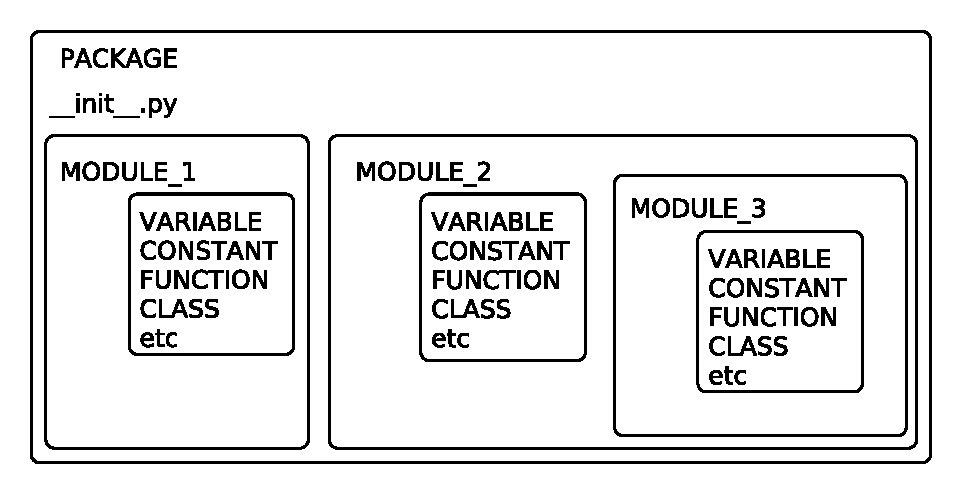
\includegraphics[scale=0.7]{pi_package_module_entity.pdf}
\caption{\label{fig:label}Python modules can be organised withing one package. A module can be placed under another module.}
\end{figure}
During first import of mdule, Python translate code from the module into \textbf{semi-compiled} format (it is not binary format) inside the \textbf{pyc} files and deploys these files into the \textbf{\_\_pycache\_\_} directory located in the module home directory. Imported module is \textbf{implicitly executed}. This is why \textbf{\_\_name\_\_=='\_\_main\_\_'} condition is used to eliminate execution durign import, and allowing to execute module during direct call. Note that in case of multiple imports of the same module, only the first import is performing by Python, other imports are silently skipping.
\paragraph{}
When importing a module or an entity from module which does not exist, an \textcolor{pythonerror}{ImportError} exception is raised.

\subsection{Namespaces and Scopes}
\textbf{Scope} and \textbf{Namespace} are corelated topics. Namespace is simply a dictionary mapping names to values. This dictionary is kind of lookup table used by Python interpreter when executing code to determine available objects (variable names, function names etc). And if they exist, the interpreter uses their values otherwise returns \textcolor{pythonerror}{NameError}. Scope according to Python definition is a textual region of a Python program where a namespace is directly accessible.
\paragraph{}
In Python we can distinguish four types of namespaces:
\begin{itemize}
\item Build-in - contains names of all build-in objects like: int, bool, list, class, ZeroDivisionError, ArithmeticError, \_, \_\_doc\_\_ etc. This scope is loading always when running script or opening interactive Python session. 
\item Global - contains all entities names created on top of module.
\item Nested (non-local) - this scope exists with nested functions, and contains object names created in enclosing function (function containing another function).
\item Local - contains entities created as part of function or lambda expression. Each call of such function or expression creates one local individual namespace (does not matter if you call multiple different function, the same function multiple times or call recurrent function).
\end{itemize}
For better understanding check following examples.
\begin{lstlisting}[style=pystyle]
# Below are 3 variables in global scope of module
variable_a = 1
variable_b = 2
variable_c = {"key1": variable_a, "key22": 22}


def function1(parameter):
	# The same variable names as local variables
    variable_a = 11
    variable_b = 2
    print(f"F1 variable_a {variable_a} ID {id(variable_a)}")
    print(f"F1 variable_b {variable_b} ID {id(variable_b)}")
    print(f"F1 parameter {parameter} ID {id(parameter)}")
    def sub_function1():
        variable_a = 111
        print(f"SUBF1 variable_a {variable_a} ID {id(variable_a)}")
        print(f"SUBF1 variable_b {variable_b} ID {id(variable_b)}")
        print(f"SUBF1 parameter {parameter} ID {id(parameter)}")
    sub_function1()

print(f"variable_a {variable_a} ID {id(variable_a)}")
print(f"variable_b {variable_b} ID {id(variable_b)}")
print(f"variable_c {variable_c} ID {id(variable_c)}")
# Produces
# variable_a 1 ID 140427234640112
# variable_b 2 ID 140427234640144
# variable_c {'key1': 1, 'key22': 22} ID 140427216021504

function1(1)
# Produces
# F1 variable_a 11 ID 140427234640432 - local scope, variable name indicate on newly created object with 11 value
# F1 variable_b 2 ID 140427234640144 - local scope, variable name indicate on object containing value 2, defined in global scope
# F1 parameter 1 ID 140427234640112 - local scope, variable name indicate on object containing value 1 also defined in global scope
# SUBF1 variable_a 111 ID 140427234643632 - local scope, variable name indicate on new object defined in namespace with value 111
# SUBF1 variable_b 2 ID 140427234640144 - local scope, variable name indicate on previously defined object with value 
# SUBF1 parameter 1 ID 140427234640112
\end{lstlisting}
The function1 contains the same variable names as global variable names. But function1 is defined in different scope. And inside function1 is defined another sub\_function1, which defines one more level of isolation. During function1 invocation a namespace is creating with parameter, variable\_a, variable\_b and sub\_function1 names. And later, during execution during sub\_function1 invocation another namespace is creating with varible\_a which is different than variable\_a from global scope and variable\_a from enclosing (function1) scope. When function is exiting (returning) namespaces disapear.

\subsubsection{Global}
\paragraph{Global} keyword is used in functions. It allows to overwrite global variable from function level.
\begin{lstlisting}[style=pystyle]
variable_a = 1

def function():
    global variable_a
    variable_a = 11
    print(f"F variable_a {variable_a} ID {id(variable_a)}")

print(f"variable_a {variable_a} ID {id(variable_a)}")
function()
print(f"variable_a {variable_a} ID {id(variable_a)}")
# Produces
# variable_a 1 ID 139973624856816
# F variable_a 11 ID 139973624857136
# variable_a 11 ID 139973624857136 - value of global variable has been changed from 1 to 11
\end{lstlisting}

\subsubsection{Nonlocal}
\paragraph{Nonlocal} keyword is used in nested functions. It allows to overwrite variable from enclosing function by nested function.
\begin{lstlisting}[style=pystyle]
variable_a = 1

def function():
    variable_a = 11
    print(f"F variable_a {variable_a} ID {id(variable_a)}")
    def sub_function():
        nonlocal variable_a
        variable_a = 111
        print(f"SUBF variable_a {variable_a} ID {id(variable_a)}")
    sub_function()
    print(f"F variable_a {variable_a} ID {id(variable_a)}")

print(f"variable_a {variable_a} ID {id(variable_a)}")
function()
# Produces
# variable_a 1 ID 139661491044592
# F variable_a 11 ID 139661491044912
# SUBF variable_a 111 ID 139661491048112 
# F variable_a 111 ID 139661491044912 - value of variable from enclosing function has been changed from 11 to 111 thanks to nonlocal keyword
\end{lstlisting}

\subsection{Creating Modules}
\paragraph{}
First line of module can contain istruction for Unix like OS, determinig how the module Python code should be launched. This line starts wiht \textbf{\#!} which is called \textbf{shebang, shabang, hasbang, poundbang or hashpling}. It has no effect under Windows OS.
\paragraph{}
Python search modules based on paths (locations) defined in system variable \textbf{PATH}, which is actually a list of Python modules locations. Access to this variable is possible from Python script using the sys module: \textbf{sys.path}. Creating our own module we can update this path variable to inform Python where to look.
\begin{lstlisting}[style=pystyle]
# Example of updating system PATH with custom module location C:/Python/custom_files
import sys
sys.path.append("C:/Python/custom_files") 
\end{lstlisting}


\subsection{\_\_pycache\_\_}
When Python import modules in another module, it first prepare a specific semi-complied files of imported modules. These files are placed in \_\_pycache\_\_ directory, and have following naming convention: \textbf{module\_name.cpython-xy.pyc}, where x and y determines python version (3.10 x=3, y=10). There precompiled files are tracked automatically by Python and updated when necessary.  


\subsection{\_\_name\_\_}
Special conditional check is used to prevent running module as standalone file when it is importing to another one module.
\begin{lstlisting}[style=pystyle]
# my_module.py

if __name__ == "__main__":
	print("This is run when my_module is executing alone")
else:
	print("This is run when my_module is importing")
	
# main.py`
import my_module

if __name__ == "__main__":
	print("This is run when main is executing alone")
else:
	print("This is run when main is importing")
\end{lstlisting}
The \_\_name\_\_ special variable keeps "\_\_main\_\_" content when it is executing directly, otherwise it keeps module name. This mechanism can be used to run test for module, when it is executing directly.
Third mechanism can be used to prevent run a module standalone.
\begin{lstlisting}[style=pystyle]
import sys

if __name__ == "__main__":
    print "Exiting!"
    sys.exit()
\end{lstlisting}

\subsection{Zip import}
Python allows to import modules directry from zip files. Assuming we get a package in form mypackag.zip and stored in somewhere in our OS. It is possible to import it as whole and access separata modules from this packages, we only have to know the file structure of the mypackage.zip. 
\begin{lstlisting}[style=pystyle]
# Add zip module to python path
import sys
sys.path.append("path/to/the/mypackage.zip")

# Import modules from zip container
# Assume the mypackage.zip have structure
# module1.py
# utils/util1.py
# src/other/module2.py
import module1
import util.util1
import src.other.module2
\end{lstlisting}
Updating a \textbf{path} Python is informed to use non standard package directory.

\subsection{Private Module Elements}
Python has no possibility to make object private inside module. Any entity created in module is visible and accessible after import. But there is a convention  to instruct users that a particular entity should be treated as private, by using \textbf{\_} or \textbf{\_\_} prefix before object name.

\subsection{\_\_init\_\_.py}
A Python file named \_\_init\_\_.py is design to be run when a package containing it is importing. Can be used to initialize a package. The file may be empty, but must exist.


\subsection{Modules Maintenance}
Python provides tools that help the creators of modules to publish, maintain, and take care of their code. First of all all packages and modules are organised in \textbf{centralised repository} which is called \textbf{PyPI - Python Package Index} (sometimes called Cheese Shop). And tool allowing users to access, install and maintain these modules is \textbf{pip - pip installs packages}, which is just package management system written in Python.
\paragraph{}
Pip can be provided with Python installer. But if not can be installed sepratelly, using dedicated OS package manager (apt in Debian like OS) or using internal Python mechanism(not recommended). Usually \textbf{pip} is installed for Python2 while \textbf{pip3} for Python3 (both versions of Python can coexist on the same OS, what is more muliple subversions of Python installation may coexist on the same OS).
\begin{lstlisting}[style=bash]
# Example pip installation command on Ubuntu
sudo apt install python3-pip
# Check version
pip3 --version
or
pip --version
# Upgrading pip to latest version
pip install --upgrade pip
# Check currently installed packages
pip3 list
# To see more usefull pip commands run help menu
pip3 help
# To see precise help to specific command
pip3 help list
# Show information about installed package
pip3 show package-name
# Search the pip universe for specifPython is able to check if the module's source file has been modified (in this case, the pyc file will be rebuilt) or not (when the pyc file may be run at once). As this process is fully automatic and transparent, you don't have to keep it in mind.ic topic (no longer supported in latest pip)
pip3 search opencv
\end{lstlisting}
Installation of new package by default is system-wide. To limit it only to specific user account an option \textbf{--user}
\begin{lstlisting}[style=bash]
# System-wide installation of numpy package
pip3 install numpy
# Installation limited to user account
pip3 install --user numpy
# Update already installed package to latest version
pip3 install -U numpy
# Install user selected version of numpy package
pip3 install numpy==1.1.0
\end{lstlisting}
Package uninstalling is also simple and strightforward
\begin{lstlisting}[style=bash]
# Uninstall numpy package
pip3 uninstall numpy
\end{lstlisting}

\subsection{Dependencies}
Python modules may depend on other python modules. To make the target module usable, all dependent modules need to be installed. So dependency is a phenomen when using part of software which relies on another software. Depencency may be nested (dependency hell). Fortunatelly \textbf{pip} can discover, identify, and resolve all dependencies. 


\newpage
\section{String Coding}
Computers store characters as numbers. Besides these visible to human, there are also other character groups, like \textbf{whitespaces} (space, tabulator, new line character), and \textbf{control characters} which are used to control input/output devices.
\paragraph{}
To make it work on different computers types, coding standards have been created. One of most popular is \textbf{ASCII - American Standard Code for Information Interchange}. The code provides space of 256 different characters (\url{https://en.wikipedia.org/wiki/ASCII}). What is dfinitelly worth to remember is fact that space character is under 32, A is under 65, a is under 97, and all letters are places in alphabed order. And 97 - 65 = 32.
\paragraph{}
\textbf{I18N - Internationalization} means modification of a software or related technologies so that a software can potentially handle multiple languages, customs, and so on in the world.
\paragraph{}
Classic ASCII uses \textbf{8 bits for each sign}, this means total different charactes is limited to 256. First 128 are used for standard Latin alphabet, but remaining 128 characters are not enough to collect remaining characters from different languages. \textbf{Code point} is a number which makes character (A - code point 65, space - code point 32). \textbf{Code page} is a standard for using upper 128 code points from standard ASCII to store specific national characters. There are different code points for Wester Europe, Eastern Europe, Cyrillic, Greek, Arabic etc alphabets. This results that the same code point e.g. 200 indicate C of Slavic language if ISO/IEC 8859-2 code page is used, or W Cyrillic letter if ISO/IEC 8859-5 code page is used. This means \textbf{to determine specific code point we have to know code page - and make it ambiguous}.
\paragraph{}
Better solution than code pages is a \textbf{UNICODE} which assigns unique (unabiguous) characters to more than a million codes. The first 128 Unicode code points are identical with ASCII, and the first 256 Unicode code points are identical to ISO/IEC 8859-1 code page (Wester Europen languages). Unicode only names all available characters and assigns them to planes (a group of characters of similar origin, application, or nature). The Unicode uses different ways of encoding:
\begin{itemize}
\item \textbf{UCS-4 Universal Character Set} uses 32 bits to store each character, and this standard define how to code and store the characters in memory. It uses BOM (byte order mark) is a special combination of bits announcing the encoding used by a files contents (e.g. UCS-4 or UTF-8).
\item \textbf{UTF-8 Unicode Transformation Format} is one of the most common standard for encoding and store Unicode texts (better than UCS-4 as it uses less memory). It uses as many bits for each of the code points as it really needs to represent them. All Latin characters and all ASCII standard characters occupy 8 bits. non Latin characters occupy 16 bits. CJK - China-Japan-Korea occupy 24 bits.
\end{itemize}
BOM (Byte Order Mark) is a special combination of bits announcing the encoding used by a file's contents (e.g. UCS-4 or UTF-8).


\subsection{Usefull functions}
Python by default provides functions to convert ASCII codes to integers and vice versa. 
\begin{lstlisting}[style=pystyle]
# Convert letter to integer
# 'A' -> 65
ord('A')

# Convert integer to letter
# 97 -> 'a'
chr(97) 
\end{lstlisting}



\newpage
\section{Standard Modules}
\subsection{Random Module}
\begin{lstlisting}[style=pystyle]
import random

# Random float value from 0.0 to 1.0
random.random()

# Random float value from provided range
# Returns float values from 3 to 5 range
random.uniform(3,5)

# Random int value from range
# Retuns values 1, 2 or 3
random.randint(1,3)

# Random int value from range and step
# Returns values 1 or 2
random.randrange(1, 3)
# Returns values 1 or 5: 1, 1+4, 1+4+4 = 9 (invalid)
random.randrange(1,9,4)

# Set seed for random functions. Default is empty - timestamp
random.seed()
random.seed(10)

# Choice single value from collection
# Select 1 element from list
random.choice([1,2,3,4,5])

# Choice one or more elements from list. Weights available
# Select 1 element from list
random.choices([1, 2, 3, 4, 5]) 
# Select 2 elements from list
random.choices([1, 2, 3, 4, 5], k=2)
# Select 1 element from list with provided weights. Weight list must be the same length as element list. For this example 3rd element (value 4) will always be selected
random.choices([1, 2, 3, 4, 5], [0, 0, 0, 1, 0])

# Sample from collection
# Get sample of 2 elements from population 1,2,3,4,5 where element 1 i repeated 4 times, element 2 i repeated 1 time and elements 3,4,5 are not preset. So the results will always contain element 1 or 2 from 1,2,3,4,5 list
random.sample([1,2,3,4,5], counts=[4,1,0,0,0], k=2)
# Which is equivalent to
random.sample([1,1,1,1,2], k=2)
# Important thing is the total number of elements in counts (sum of counts) must be equal or grater than lenght of samples list. In example above, replacing counts=[4,1,0,0,0] with counts=[3,1,0,0,0] will produce ValueError.

# Random int value from number of bits
# For 3 bits returns integers in range 0 to 7
random.getrandbits(3)

# Random bytes
# For 2 generates random 2 bytes, e.g. b'%\x8e
random.randbytes(2) 

# Change elements in collection in place
# For l=[1,2,3,4,5] return 5 element list, e.g. [3,5,2,4,1]
random.shuffle(l)	
\end{lstlisting}

\subsection{Math Module}
\begin{lstlisting}[style=pystyle]
import math

# Access some common constant entities
math.e		# 2.718281
math.pi		# 3.141592
math.tau	# 6.283185
math.inf	# float('inf')
math.nan	# float('nan')

# Ceil - round up to int
math.ceil(-1.1)		# -1
math.ceil(1.1)		# 2

# Floor - round down to int
math.floor(3.3)		# 3
math.floor(-3.3)	# -4

# Trunc - round to the int part
math.trunc(3.3)		# 3
math.trunc(-3.3)	# -3

# Close - returns True if values are close, otherwise False
# E.g. check values differs no more than 5%
math.isclose(100, 94.999, rel_tol=0.05)	# False
math.isclose(100, 95, rel_tol=0.05)		# True
# E.g. check values differs no more then 2 absolute value
math.isclose(100, 98, abs_tol=2)	# True
math.isclose(100, 97.5, abs_tol=2)	# False

# Sum collection of numbers without loss of precission
math.fsum([.1,.1,.1])		# 0.3

# Square root of number
math.sqrt(16)	# 4.0

# Power
math.pow(3,2)	# 9.0

# Return e raised to the power of x
math.exp(1)			# 2.718281828459045

# Logarithms
math.log(math.e)	# 1.0
math.log2(2)		# 1.0
math.log10(10)		# 1.0

# Trigonometric functions
x=0.5
math.sin(x)
math.cos(x)
math.tan(x)
math.asin(x)
math.acos(x)
math.atan(x)

# Angular conversions
math.degrees(math.pi)	# 180.0 degrees
math.radians(180)		# 3.141592653589793 rad

# Hyperbolic functions - are analogs of trigonometric functions that are based on hyperbolas instead of circles.
x=0.5
math.sinh(x)
math.cosh(x)
math.tanh(x)
math.asinh(x)
math.acosh(1)
math.atanh(x)

# Returns evaluation of sqrt((x * x + y * y)). Triangle x1 is a length of 1 arm, x2 is a lenght of 2nd arm. The hypot calculate lenght of the 3rd arm - hypotenuse
math.hypot(x1, x2)
\end{lstlisting}

\subsection{Platform Module}
Access hardware, system and python specific information.
\begin{lstlisting}[style=pystyle] 
import platform

# Access HW architecture of processor
platform.architecture()	# Returns e.g. ('64bit', 'ELF')

# Access machine type
platform.machine()		# Returns e.g. 'x86_64'

# Return processor information
platform.processor()	# Returns e.g. 'x86_64'

# Access name of computer
platform.node()			# Returns e.g. 'dupa-T440p'

# Return platform information
platform.platform()		# Returns string with OS information
platform.system()		# Returns e.g. 'Linux'

# Return collected information about system, node etc.
platform.uname()

# Return information about installed Python
platform.python_compiler()	# Returns e.g. 'GCC 7.5.0'
platform.python_branch()
platform.python_implementation()	# Returns e.g.'CPython'
platform.python_revision()
platform.python_version()	# Returns e.g. '3.10.10'
platform.python_version_tuple() # Returns e.g. ('3', '10', '10')
\end{lstlisting}

\subsection{Os Module}
Module to use operating system functionality. Provide functionalities to operate on file system (paths, directories, files) etc.
\begin{lstlisting}[style=pystyle]
import os

# Print information about current OS
# sysname - name of the operating system
# nodename - machine name on the network
# machine - hw identifier
# release - operating system release
# version - operating system versuion
os.uname()
# posix.uname_result(sysname='Linux', nodename='anana-T440p',  release='4.15.0-210-generic', version='#221-Ubuntu SMP Tue Apr 18 08:32:52 UTC 2023', machine='x86_64')
# Accessing each element separatelly
os.uname().sysname	#'Linux'
os.uname().nodename	#'anana-T440p'
os.uname().release	#'4.15.0-210-generic'
os.uname().version	#'#221-Ubuntu SMP Tue Apr 18 08:32:52 UTC 2023'
os.uname().machine	#'x86_64'

# Check type of OS
# posix - Linux like system
# nt - Windows
# java - Juthon machine
os.name

# Print content of current directory
# returns likst of element sin directory without .. and .
os.listdir()

# Print absolute path of current direcotry. 
os.getcwd()

# Create directory
# relative path
os.mkdir("new_dir")
# absolute path
os.mkdir("/usr/my_space/new_dir")
# If the file exist, method returns FileExistsError
# create path of directories. This method allows to configure specific access right to creating directory
os.makedirs("ala/ma/kota") # creates 2 directories: ala, ma, kota

# Remove directory
# relative path
os.rmdir("ma")
# absolute path
os.rmdir("/usr/my_space/new_dir")
# remove direcotry with its content (files or other directories)
os.removedirs("ala/ma/kota")
 
# Switch between directories
os.chdir("..")		# one directory up
os.chdir("../..")	# two directories up

# Call any system function. If operation is successfull return code is 0 (in case of Linux). Otherwise, the specific error code tells you what went wrong.
os.system("ls -al")
os.system("mkdir lala")
os.system("rm -r lala") 

# Construct correct paths in file system
# Join two paths
os.path.join(os.getcwd(), "wata")	# '/home/anana/moje/projekty/python/pythongniewomirkurs/katalogdousuniecia/kaszanka/wata'
# Split path - from provided path, split the last component, and remaining path without it, and returs as tuple
os.path.split(os.getcwd())	# ('/home/anana/moje/projekty/python/pythongniewomirkurs/katalogdousuniecia', 'kaszanka')
# Print absolute path of current positon
os.path.abspath(".")
# Check it is a directory
os.path.isdir(".")		# True
# Check it is a file
os.path.isfile(".")		# False
# check it is a link
os.path.islink()		# False

# Walk throught directories and get information about files
for paths, dirs, files in os.walk("."):
    print(f"files {files}, dirs {dirs}, paths {paths}")

# Provide methods to operate on file (open, write, read, close)
fd = os.open("test.txt", os.O_RDWR|os.O_CREAT)
os.write(fd, str.encode("Czesc i Pa"))	# 10 number of characters
os.close(fd)

\end{lstlisting}

\textbf{Relative path} - is a short path, starting from current directory. \textbf{Absolute path} - is a long path, starting from root directory.

\subsection{Time Module} \label{time:0}
Provides methods to represent and manipulate time as float, string or structures. First lets learn few definitions which are crucial to understand time module utilities:
\begin{itemize} \label{time:1}
\item \textbf{epoch} - it is starting point against which time is measuring. Most popular epoch is: Jan 1 1970 UTC, and it is used on majority OS.
\item \textbf{timezone} - it is a region of World that conforms a standardized time. Timezones are expressed using possitive or negative offsets from UTC.
\item \textbf{UTC} - Coordinated Universal Time - tiem standard.
\item \textbf{GTM} - Greenwitch Mean Time - time zone officially used in some contries.
\item \textbf{local time} - it is time in your location.
\item \textbf{daylight saving time} - it a 1 hour shift (negative or possitive) in current timezone, to make a kind of time adjustment during summer and winter period.
\item \textbf{STRUCT\_TIME} - named tuple, containing 9 fields, representing date, time, daylight and extra information abot time zone.
\end{itemize}

\begin{lstlisting}[style=pystyle] 
import time

# LOCALTIME as SECONDS
time.time()	#1697905608.2663414

# TUPLE to STRUCT_TIME
my_time_tuple = (1999, 10, 30, 23, 10, 60, 1, 1, 1)
my_time = time.struct_time(my_time_tuple)
print(my_time)
#time.struct_time(tm_year=1999, tm_mon=10, tm_mday=30, tm_hour=23, tm_min=10, tm_sec=60, tm_wday=1, tm_yday=1, tm_isdst=1)

# UTC, STRUCT_TIME to SECONDS
import calendar
calendar.timegm(my_time)	# 941325060

# LOCALTIME, STRUCT_TIME to SECONDS
time.mktime(my_time)	# 941317860.0

# UTC, SECONDS to STRUCT_TIME
time.gmtime(123)
#time.struct_time(tm_year=1970, tm_mon=1, tm_mday=1, tm_hour=0, tm_min=2, tm_sec=3, tm_wday=3, tm_yday=1, tm_isdst=0)

# LOCALTIME, SECONDS to STRUCT_TIME
time.localtime()
#time.struct_time(tm_year=2023, tm_mon=10, tm_mday=21, tm_hour=18, tm_min=24, tm_sec=34, tm_wday=5, tm_yday=294, tm_isdst=1)

# STRING to STRUCT_TIME
time.strptime("2023 10 - 1 2 3", "%Y %m - %H %M %S")
#time.struct_time(tm_year=2023, tm_mon=10, tm_mday=1, tm_hour=1, tm_min=2, tm_sec=3, tm_wday=6, tm_yday=274, tm_isdst=-1)

# SECONDS to STRING
time.ctime(123)	#'Thu Jan  1 01:02:03 1970'

# STRUCT_TIME to STRING
time.asctime(my_time)	#'Tue Oct 30 23:10:60 1999'

# LOCALTIME formated STRING
time.strftime("%Y - %M - %D")	#'2023 - 47 - 10/21/23'

# STRUCT_TIME to formated STRING
time.strftime("%Y - %M - %D", my_time)	#'1999 - 10 - 10/30/99'

# susped execution
time.sleep(0.012)

# measurig performance - process_time doeas not take into account sleep time, while perf_counter calculate wole execution time.
start = time.process_time() 
time.sleep(0.1)
stop = time.process_time()
print(start-stop)		#0.0

start = time.perf_counter() 
time.sleep(0.1)
stop = time.perf_counter()
print(start-stop)		#-0.11232290000043577

\end{lstlisting}

\subsection{Datetime Module}
Provides methods to represent and manipulate dates and times. Refer to \ref{time:1} few useful definitions first. This module introduces olso two more definitions:
\begin{itemize}
\item \textbf{naive} - means the date and time may not reflect actual geopolitical values.
\item \textbf{aware} - when information like \textit{tzinfo is not None} and \textit{tzinfo.utcoffset does not return None} the date and time reflects actual geopolitical values. 
\item \textbf{weekday} - from Monday=0 to Sunday=6.
\item \textbf{isoweekday} - from Monday=1 to Sunday=7.
\end{itemize}
Naive and aware definitions are valid only for datetime.datetime and datetime.time.

\begin{lstlisting}[style=pystyle] 
import datetime as dt

# DATE from constructor
data = dt.date(1999, 2, 3)
print(data)		#1999-02-03

# DATE from today method
data = dt.date.today()
data.year		#2023
data.month		#10
data.day		#22

# DATE from SECONDS
data = dt.date.fromtimestamp(1697890111) 
data.month	#10
data.year	#2023
data.day	#21

# DATE from ISOFORMAT
# year, month, day
dt.date.fromisoformat('2019-12-04')	#datetime.date(2019, 12, 4)
dt.date.fromisoformat('0001-01-04')	#datetime.date(1, 1, 4)

# DATE from ISOCALENDAR
# year, weeknumber, weekday
dt.date.fromisocalendar(2019, 12, 4)	#datetime.date(2019, 3, 21)
dt.date.fromisocalendar(2019, 50, 1)	#datetime.date(2019, 12, 9)

# Replace year, month or day in given DATE
data = dt.date(1999,4,8)	#datetime.date(1999, 4, 8)
data.replace(day=1)			#datetime.date(1999, 4, 1)

# Return DATE as STRUCT_TIME
data = dt.date(1999,4,8)
data.timetuple()
# time.struct_time(tm_year=1999, tm_mon=4, tm_mday=8, tm_hour=0, tm_min=0, tm_sec=0, tm_wday=3, tm_yday=98, tm_isdst=-1)

# DATE access and representation methods
data.weekday()		#3
data.isoweekday()	#4
data.isoformat()	#'1999-04-08'
data.isocalendar()	#datetime.IsoCalendarDate(year=1999, week=14, weekday=4)
data.month			#4
data.day			#8
data.year			#1999
data.ctime()		#'Thu Apr  8 00:00:00 1999'




\end{lstlisting}


\newpage
\section{Examples}
\subsection{Data Sorting}
\subsubsection{Bubble Sort}
	Bubble Sorting is a simple sorting method with O(n2) time complexity. The idea bases of comparing two next elements and swapping them if the order is incorrect. The end of the sotrting is when after iteration there are not elements to be switched. Example of implementation is shown below:
\begin{lstlisting}[style=pystyle]
import random
import time


def bubble(data_to_sort) -> list:
    # define flag to monitor if swap has palace or not
    switched_flag = True
    # repeat iteration as soon as swap has pace before
    while switched_flag:
        switched_flag = False
        # as we operate on current and next element, iteration is limited to next to the last element.
        for index in range(len(data_to_sort)-1):
            if data_to_sort[index] > data_to_sort[index+1]:
                # perform swap in Python manner
                data_to_sort[index], data_to_sort[index+1] = data_to_sort[index+1], data_to_sort[index]
                switched_flag = True
    return data_to_sort


if __name__ == '__main__':
    # generate list of 10k random integers from -1e6 to 1e6
    list_to_be_sorted = [random.randint(-1000000, 1000000) for _ in range(10000)]
    # measure execution time
    time_start = time.time()
    bubble(list_to_be_sorted)
    print(round(time.time() - time_start, 6), "[s]")
\end{lstlisting}

\subsubsection{LCD}	
Print integer number as 7-segment LCD.
\begin{lstlisting}[style=pystyle]
def print_lcd(number):
    
    lcd = [["### ",
            "# # ",
            "# # ",
            "# # ",
            "### "],
           ["  # ",
            "  # ",
            "  # ",
            "  # ",
            "  # "],
           ["### ",
            "  # ",
            "### ",
            "#   ",
            "### "],
           ["### ",
            "  # ",
            "### ",
            "  # ",
            "### "],
           ["# # ",
            "# # ",
            "### ",
            "  # ",
            "  # "],
           ["### ",
            "#   ",
            "### ",
            "  # ",
            "### "],
           ["### ",
            "#   ",
            "### ",
            "# # ",
            "### "],
           ["### ",
            "  # ",
            "  # ",
            "  # ",
            "  # "],
           ["### ",
            "# # ",
            "### ",
            "# # ",
            "### "],
           ["### ",
            "# # ",
            "### ",
            "  # ",
            "### "]]
     
    number_str = str(number)
    for line in range(5):
        for char in number_str:
            print(lcd[int(char)][line], end="")
        print()
        
print_lcd(42878248264)
\end{lstlisting}      

\subsubsection{Modified Ceasar Cipher}
\begin{lstlisting}[style=pystyle]
u_min = ord("A")
u_max = ord("Z")
l_min = ord("a")
l_max = ord("z")
    
def coder(value, kod_max, kod_min):
    decimal = value // (kod_max + 1)
    fract = value % (kod_max + 1)
    if decimal:
        return fract + kod_min
    return fract

def ceasar_cipher_2():
    message = input("Dawaj data: ")
    shift = int(input("Dawaj kodowanie: "))
    text_coded = ""
    for c in message:
        if not c.isalpha():
            text_coded += c
        else:
            if c.isupper():
                text_coded += chr(coder(ord(c)+shift, u_max, u_min))
            else:
                text_coded += chr(coder(ord(c)+shift, l_max, l_min))
    print(text_coded)
                
ceasar_cipher_2()
\end{lstlisting}

\subsubsection{Cartesian Distance}
Calculate distance between current and new point on cartesian area.
\begin{lstlisting}[style=pystyle]
class P:
    def __init__(self, x=0.0, y=0.0):
        self.x = x
        self.y = y
    def distance_last_new(self, x, y):
        dist = math.hypot(abs(self.x - x), abs(self.y - y))
        print(f"New position {x},{y}. Distance from old {self.x},{self.y} = {dist}")
        self.x = x
        self.y = y
p=P()
p.distance_last_new(1,1)
#New position 1,1. Distance from old 0.0,0.0 = 1.4142135623730951
\end{lstlisting}


\end{document}
